\documentclass[a4paper, twoside]{article}

%% Language and font encodings
\usepackage[english]{babel}
\usepackage[T1]{fontenc}

%% Sets page size and margins
\usepackage[a4paper,top=3cm,bottom=3cm,left=3cm,right=3cm,marginparwidth=1.75cm]{geometry}
\usepackage{array}

%% Useful packages
\usepackage{amsmath}
\usepackage{graphicx}
\usepackage[colorlinks=true, allcolors=black]{hyperref}
\usepackage[utf8]{inputenc}
\usepackage{fancyhdr}
\usepackage{capt-of}
\usepackage{listings}
\usepackage{xcolor}
\usepackage{setspace}
\usepackage{tocloft}
\usepackage{float}

%% Header / Footer
\pagestyle{fancy}
\fancyhf{}
\fancyhead[LE,RO]{Binge -- Video Streaming Platform}
\fancyhead[RE,LO]{DS Lab Final Project}
\fancyfoot[LE,RO]{\thepage}
\renewcommand{\headrulewidth}{2pt}
\renewcommand{\footrulewidth}{1pt}

%% Table of contents formatting
\cftsetindents{section}{0em}{2em}
\cftsetindents{subsection}{0em}{2em}
\renewcommand\cfttoctitlefont{\hfill\Large\bfseries}
\renewcommand\cftaftertoctitle{\hfill\mbox{}}

%% Code listing style
\lstset{
    basicstyle=\ttfamily\small,
    keywordstyle=\color{blue},
    commentstyle=\color{gray},
    stringstyle=\color{orange},
    breaklines=true,
    frame=single,
    backgroundcolor=\color{gray!10}
}

\title{Binge: Video Streaming Platform}
\author{[Your Name] \\ Roll No: [Your Roll No]}

\begin{document}
\begin{titlepage}

\newcommand{\HRule}{\rule{\linewidth}{0.5mm}}

%----------------------------------------------------------------------------------------
%	LOGO SECTION
%----------------------------------------------------------------------------------------
\centering

\includegraphics[width=5cm]{Figures/uet_logo.png}\\[1cm]

%----------------------------------------------------------------------------------------

\center

%----------------------------------------------------------------------------------------
%	HEADING SECTIONS
%----------------------------------------------------------------------------------------
\textbf{\Large Department of Computer Science}\\[0.5cm]
\textbf{\LARGE University of Engineering and Technology Lahore Pakistan}\\[1.5cm]
\vfill

%----------------------------------------------------------------------------------------
%	TITLE SECTION
%----------------------------------------------------------------------------------------
\makeatletter
\HRule \\[0.4cm]
{ \huge \bfseries \@title}\\[0.4cm]
\HRule \\[1.5cm]

%----------------------------------------------------------------------------------------
%	AUTHOR SECTION
%----------------------------------------------------------------------------------------

\begin{minipage}{0.4\textwidth}
\begin{flushleft} \large
\emph{Submitted by:}\\
\@author
\end{flushleft}
\end{minipage}
~
\begin{minipage}{0.4\textwidth}
\begin{flushright} \large
\emph{Submitted to:} \\
Mr. Nazeef Ul Haq \\[1.2em]
\end{flushright}
\end{minipage}\\[2cm]
\makeatother

%----------------------------------------------------------------------------------------
%	DATE SECTION
%----------------------------------------------------------------------------------------

{\large \today}\\[2cm]

\vfill

\end{titlepage}

\pagenumbering{roman}
\setcounter{page}{1}

\setcounter{tocdepth}{3}
\tableofcontents
\addtocontents{toc}{~\hfill\textbf{Page}\par}

\clearpage
\listoftables
\addcontentsline{toc}{section}{List of Tables}
\clearpage
\listoffigures
\addcontentsline{toc}{section}{List of Figures}
\clearpage
\singlespacing
\pagenumbering{arabic}
\setcounter{page}{1}

% ============================================================
\section{Overview}
% ============================================================

\subsection{Description}
Binge is a full-stack video streaming web application inspired by platforms like YouTube. It allows users to watch, like, comment on, and save videos to playlists; creators to upload and manage their channels through a dedicated studio dashboard; and administrators to moderate content, manage users, and generate detailed PDF analytics reports. The platform is built using Node.js, Express, EJS templating, MySQL, and Tailwind CSS, with a focus on meaningful use of advanced database features including views, stored procedures, and triggers.

\subsection{Business Case}
Binge addresses the growing demand for content creator platforms that provide both a seamless viewing experience and powerful creator management tools. The platform can serve educational institutions, entertainment portals, or any organization looking to host and manage video content at scale. The built-in analytics and PDF reporting system gives administrators actionable insights into platform performance without requiring third-party tools.

\subsection{Motivation}
Managing video content, user engagement, and platform moderation manually is not scalable. Creators need real-time channel statistics; viewers need personalized feeds based on their subscriptions; and administrators need tools to monitor abuse, manage users, and generate reports on demand. Binge consolidates all these requirements into a single platform with clearly separated roles and a relational database designed for integrity and performance.

\subsection{Audience}
\begin{itemize}
    \item \textbf{Viewers} -- Anyone who wants to watch, like, comment on, and organize videos.
    \item \textbf{Creators} -- Content producers who upload and manage their video channels.
    \item \textbf{Administrators} -- Platform moderators who oversee users, content, and reports.
\end{itemize}

\subsection{Features}

\begin{enumerate}
    \item User registration, login, and session management
    \item Role-based access control (Viewer, Creator, Admin)
    \item Video browsing with category-based filtering
    \item YouTube-embedded video playback
    \item Like, comment, subscribe, and report functionality
    \item Watch history tracking and playlist management
    \item Creator studio dashboard with aggregated statistics
    \item Video upload, edit, and delete with tag management
    \item Admin panel with user and content moderation tools
    \item 10 on-demand PDF reports generated with PDFKit
    \item Avatar and profile photo upload via Multer
    \item Password hashing with bcryptjs
    \item Input validation via a custom Validator class
    \item Singleton Logger class writing to log files
    \item Mobile-responsive design with Tailwind CSS
\end{enumerate}

\subsection{Technology Stack}

\begin{table}[ht!]
\centering
\caption{Technology Stack}
\label{tab:TechStack}
\begin{tabular}{|l|l|}
\hline
\textbf{Layer}       & \textbf{Technology}              \\ \hline
Platform             & Web (Browser-based)              \\ \hline
Runtime              & Node.js                          \\ \hline
Framework            & Express.js                       \\ \hline
Templating Engine    & EJS (Embedded JavaScript)        \\ \hline
Styling              & Tailwind CSS (CDN) + Custom CSS  \\ \hline
Database             & MySQL 8.0                        \\ \hline
DB Driver            & mysql2 (callback-based)          \\ \hline
Authentication       & bcryptjs + express-session       \\ \hline
File Uploads         & Multer                           \\ \hline
PDF Generation       & PDFKit                           \\ \hline
\end{tabular}
\end{table}

% ============================================================
\section{Use Cases}
% ============================================================

% ------- U01 -------
\subsection{Register}
\begin{table}[ht!]
\centering
\caption{U01: Register}
\label{tab:U01}
\begin{tabular}{|>{\hspace{0pt}}m{0.122\linewidth}|>{\hspace{0pt}}m{0.839\linewidth}|}
\hline
Use Case ID & U01 \\ \hline
Name        & Register \\ \hline
Actor       & New User \\ \hline
Description & A new user creates an account by providing first name, last name, email, password, confirm password, country, and selecting a role (Viewer or Creator). The \texttt{Validator} class checks all fields before submission. If the email already exists the form re-renders with an error message. Passwords are hashed with bcryptjs before being stored in the database. \\ \hline
\end{tabular}
\end{table}

\begin{figure}[ht!]
\centering
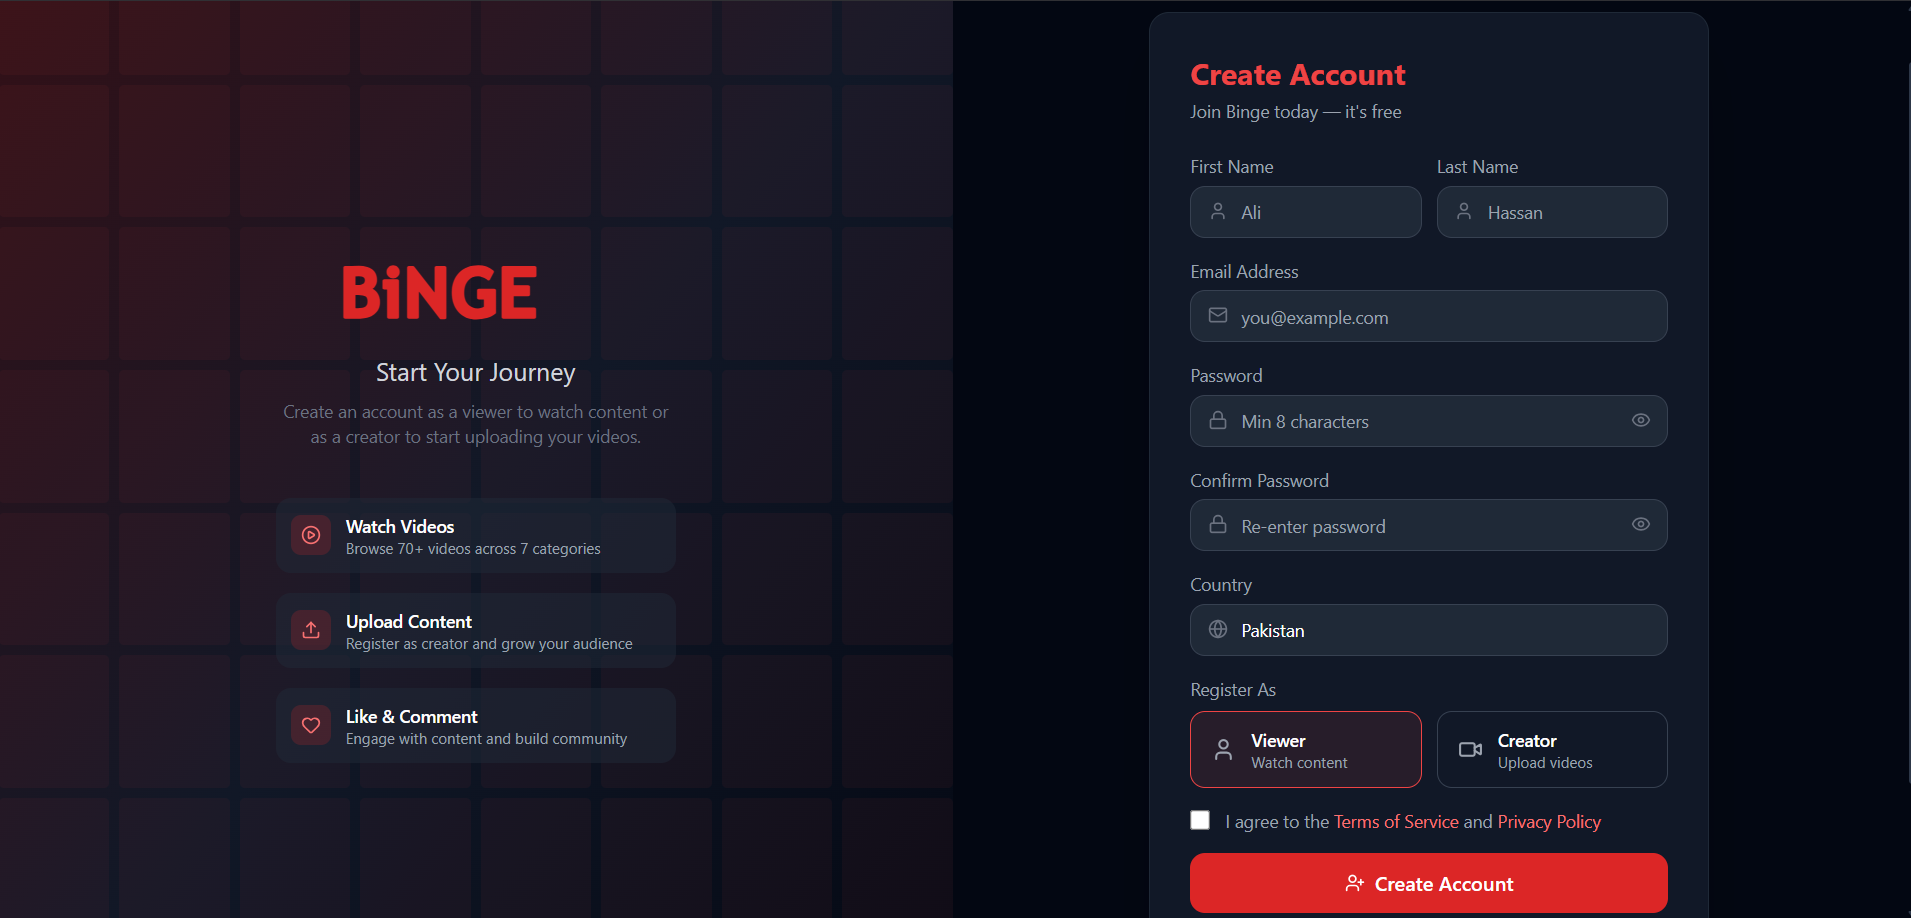
\includegraphics[width=\textwidth,keepaspectratio]{Figures/U01.png}
\caption{U01: Register Screen}
\label{fig:U01}
\end{figure}
\clearpage

% ------- U02 -------
\subsection{Login}
\begin{table}[ht!]
\centering
\caption{U02: Login}
\label{tab:U02}
\begin{tabular}{|>{\hspace{0pt}}m{0.122\linewidth}|>{\hspace{0pt}}m{0.839\linewidth}|}
\hline
Use Case ID & U02 \\ \hline
Name        & Login \\ \hline
Actor       & Registered User \\ \hline
Description & A registered user enters their email and password. The system looks up the account, verifies the bcrypt hash, and checks whether the account is active. An express-session is created storing the user's id, name, role, and avatar. The session protects all subsequent routes. On logout the session is destroyed and the user is redirected to the login page. \\ \hline
\end{tabular}
\end{table}

\begin{figure}[ht!]
\centering
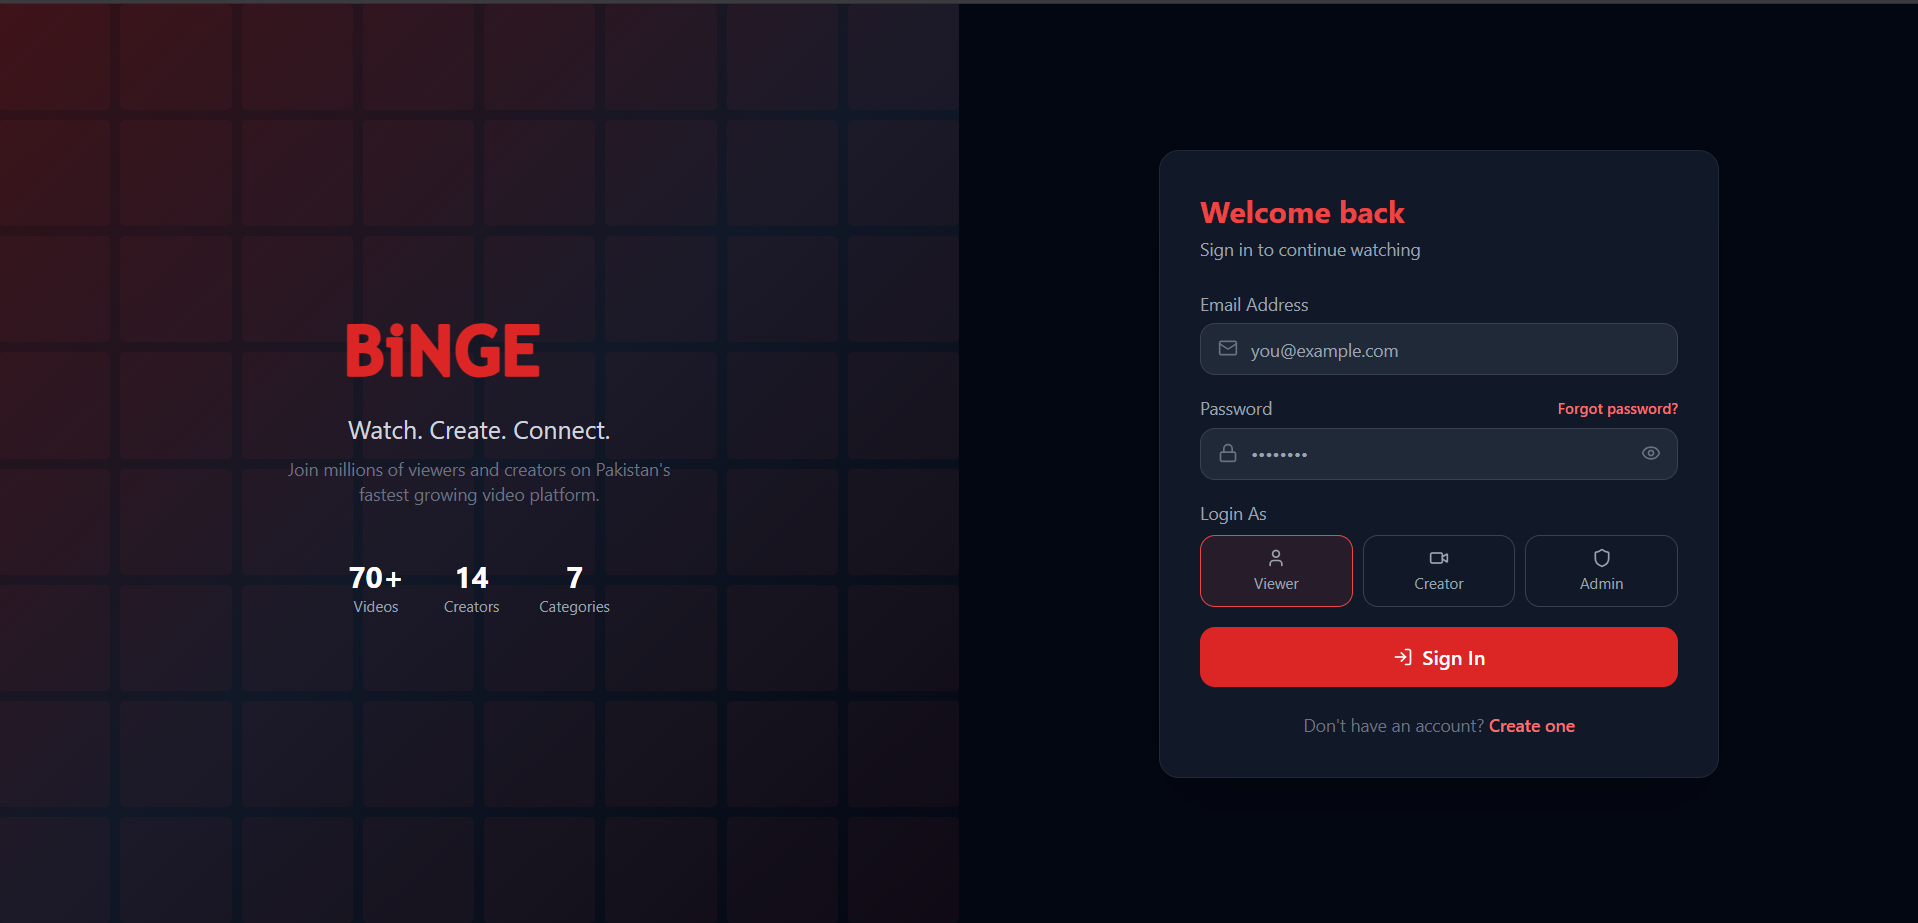
\includegraphics[width=\textwidth,keepaspectratio]{Figures/U02.png}
\caption{U02: Login Screen}
\label{fig:U02}
\end{figure}
\clearpage

% ------- U03 -------
\subsection{Browse Home Feed}
\begin{table}[ht!]
\centering
\caption{U03: Browse Home Feed}
\label{tab:U03}
\begin{tabular}{|>{\hspace{0pt}}m{0.122\linewidth}|>{\hspace{0pt}}m{0.839\linewidth}|}
\hline
Use Case ID & U03 \\ \hline
Name        & Browse Home Feed \\ \hline
Actor       & Viewer \\ \hline
Description & After login the viewer lands on the home page displaying all published videos ordered by upload date. Each video card shows the YouTube thumbnail, title, channel name, view count, and upload date. Category pills at the top allow quick filtering by content type. The page adapts from a single column on mobile to a multi-column grid on desktop. \\ \hline
\end{tabular}
\end{table}

\begin{figure}[ht!]
\centering
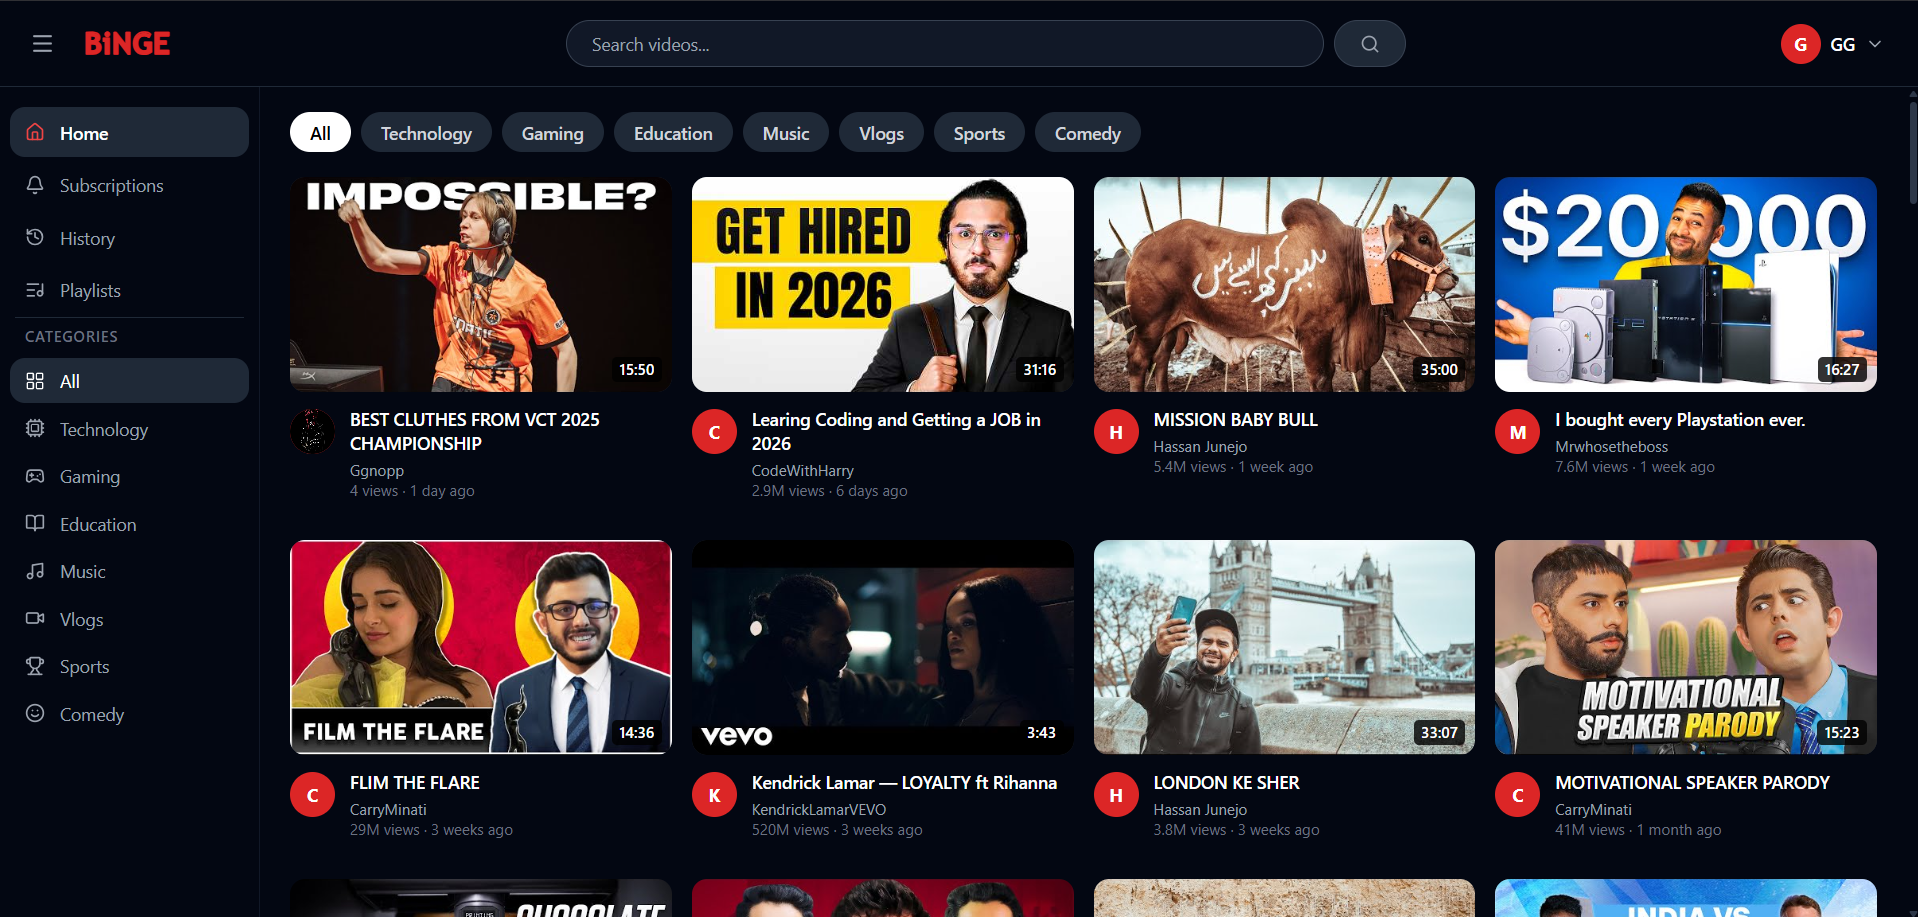
\includegraphics[width=\textwidth,keepaspectratio]{Figures/U03.png}
\caption{U03: Home Feed Screen}
\label{fig:U03}
\end{figure}
\clearpage

% ------- U04 -------
\subsection{Watch Video}
\begin{table}[ht!]
\centering
\caption{U04: Watch Video}
\label{tab:U04}
\begin{tabular}{|>{\hspace{0pt}}m{0.122\linewidth}|>{\hspace{0pt}}m{0.839\linewidth}|}
\hline
Use Case ID & U04 \\ \hline
Name        & Watch Video \\ \hline
Actor       & Viewer \\ \hline
Description & Clicking a video card opens the watch page. The watch page brings together all viewer interactions on one screen:
\begin{itemize}
    \item \textbf{Playback} -- The video URL is converted to a YouTube embed URL and rendered in an iframe. The stored procedure \texttt{sp\_RecordVideoView} is called which atomically increments the view count and inserts a \texttt{watchhistory} record in a single transaction. The \texttt{trg\_UpdateCreatorViews} trigger fires automatically from inside the SP to keep the creator's total views in sync.
    \item \textbf{Like / Unlike} -- The viewer can toggle a like. A row is inserted into or deleted from the \texttt{likes} table and the total count updates.
    \item \textbf{Subscribe / Unsubscribe} -- The viewer can subscribe or unsubscribe by clicking the channel button. This calls the stored procedure \texttt{sp\_ToggleSubscription} which atomically updates the subscription row and the creator's \texttt{TotalSubscribers} counter.
    \item \textbf{Save to Playlist} -- The viewer can add the video to any of their playlists via a dropdown.
    \item \textbf{Comments} -- The viewer can post a comment which is inserted into the \texttt{comment} table. Existing comments are shown in reverse chronological order.
    \item \textbf{Report} -- The viewer can report the video for inappropriate content. A \textit{Pending} record is created in the \texttt{report} table and appears in the admin moderation queue.
    \item \textbf{Related Videos} -- A sidebar shows other published videos from the same category.
\end{itemize} \\ \hline
\end{tabular}
\end{table}

\begin{figure}[ht!]
\centering
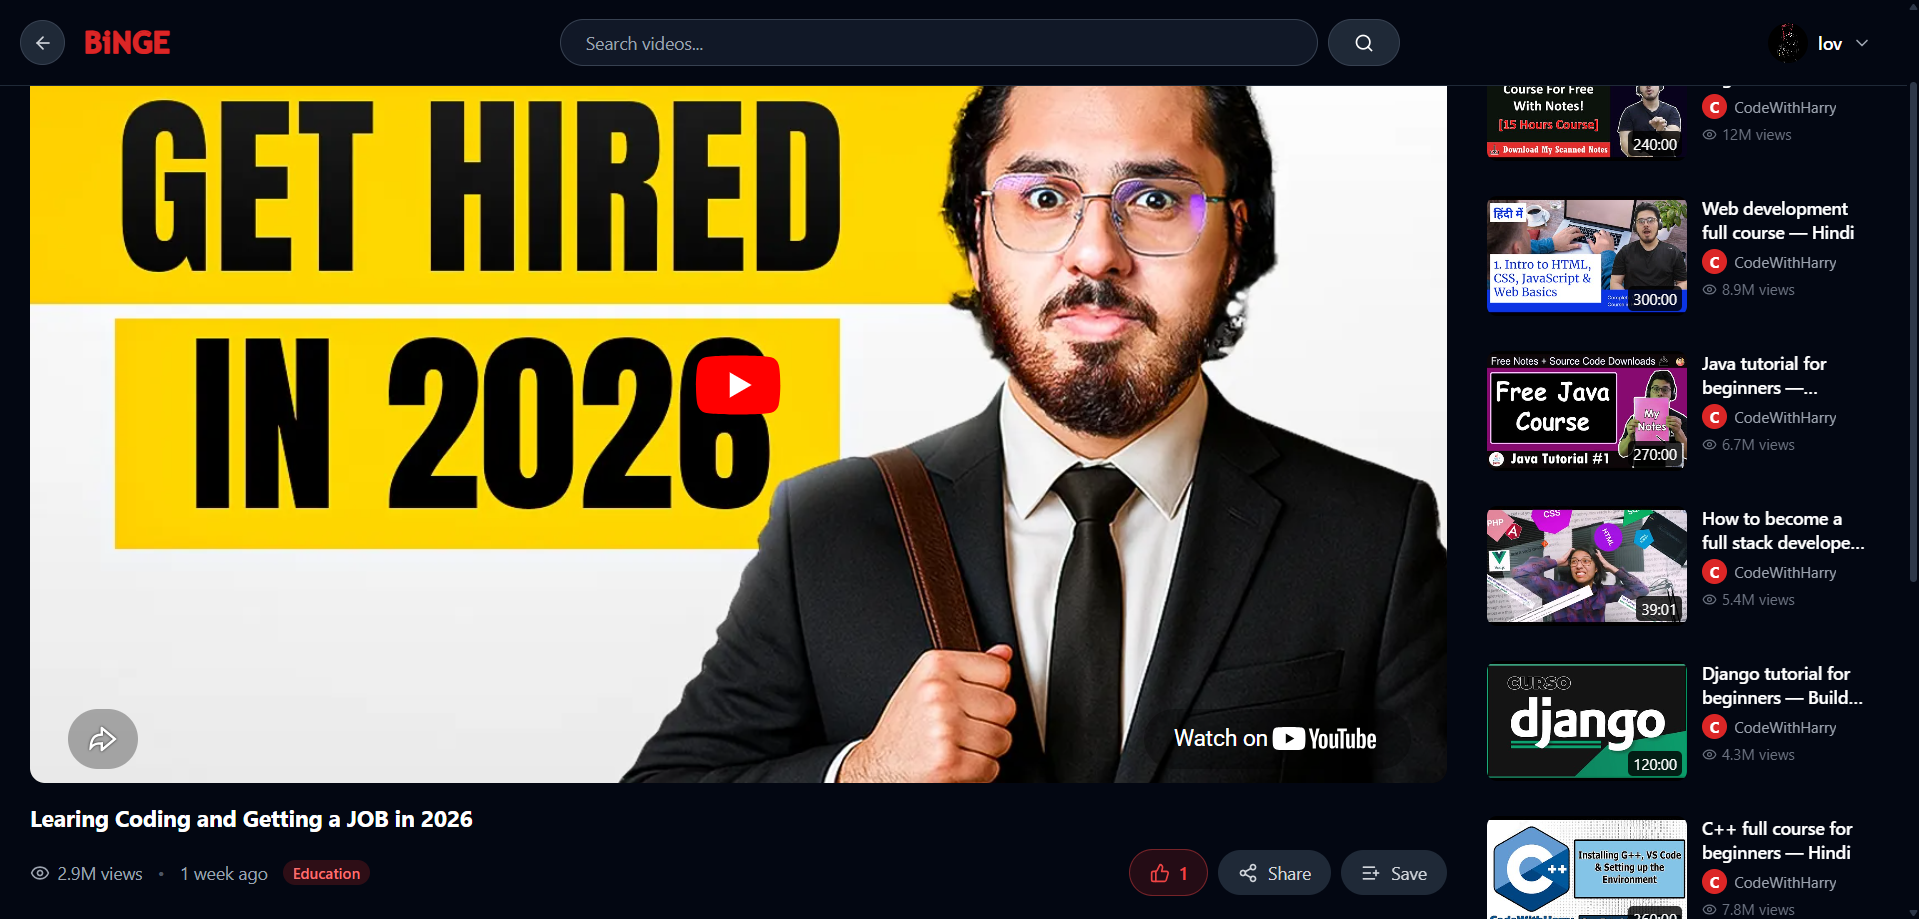
\includegraphics[width=\textwidth,keepaspectratio]{Figures/U04.png}
\caption{U04: Watch Video Screen}
\label{fig:U04}
\end{figure}
\clearpage

% ------- U05 -------
\subsection{Watch History}
\begin{table}[ht!]
\centering
\caption{U05: Watch History}
\label{tab:U05}
\begin{tabular}{|>{\hspace{0pt}}m{0.122\linewidth}|>{\hspace{0pt}}m{0.839\linewidth}|}
\hline
Use Case ID & U05 \\ \hline
Name        & Watch History \\ \hline
Actor       & Viewer \\ \hline
Description & The history page lists all videos the viewer has watched in descending order of watch time, showing title, channel, category, and completion percentage. The viewer can delete a single entry or clear the entire history at once. This data also feeds the \texttt{vw\_MonthlyWatchSummary} view which is used in the admin monthly watch PDF report. \\ \hline
\end{tabular}
\end{table}

\begin{figure}[ht!]
\centering
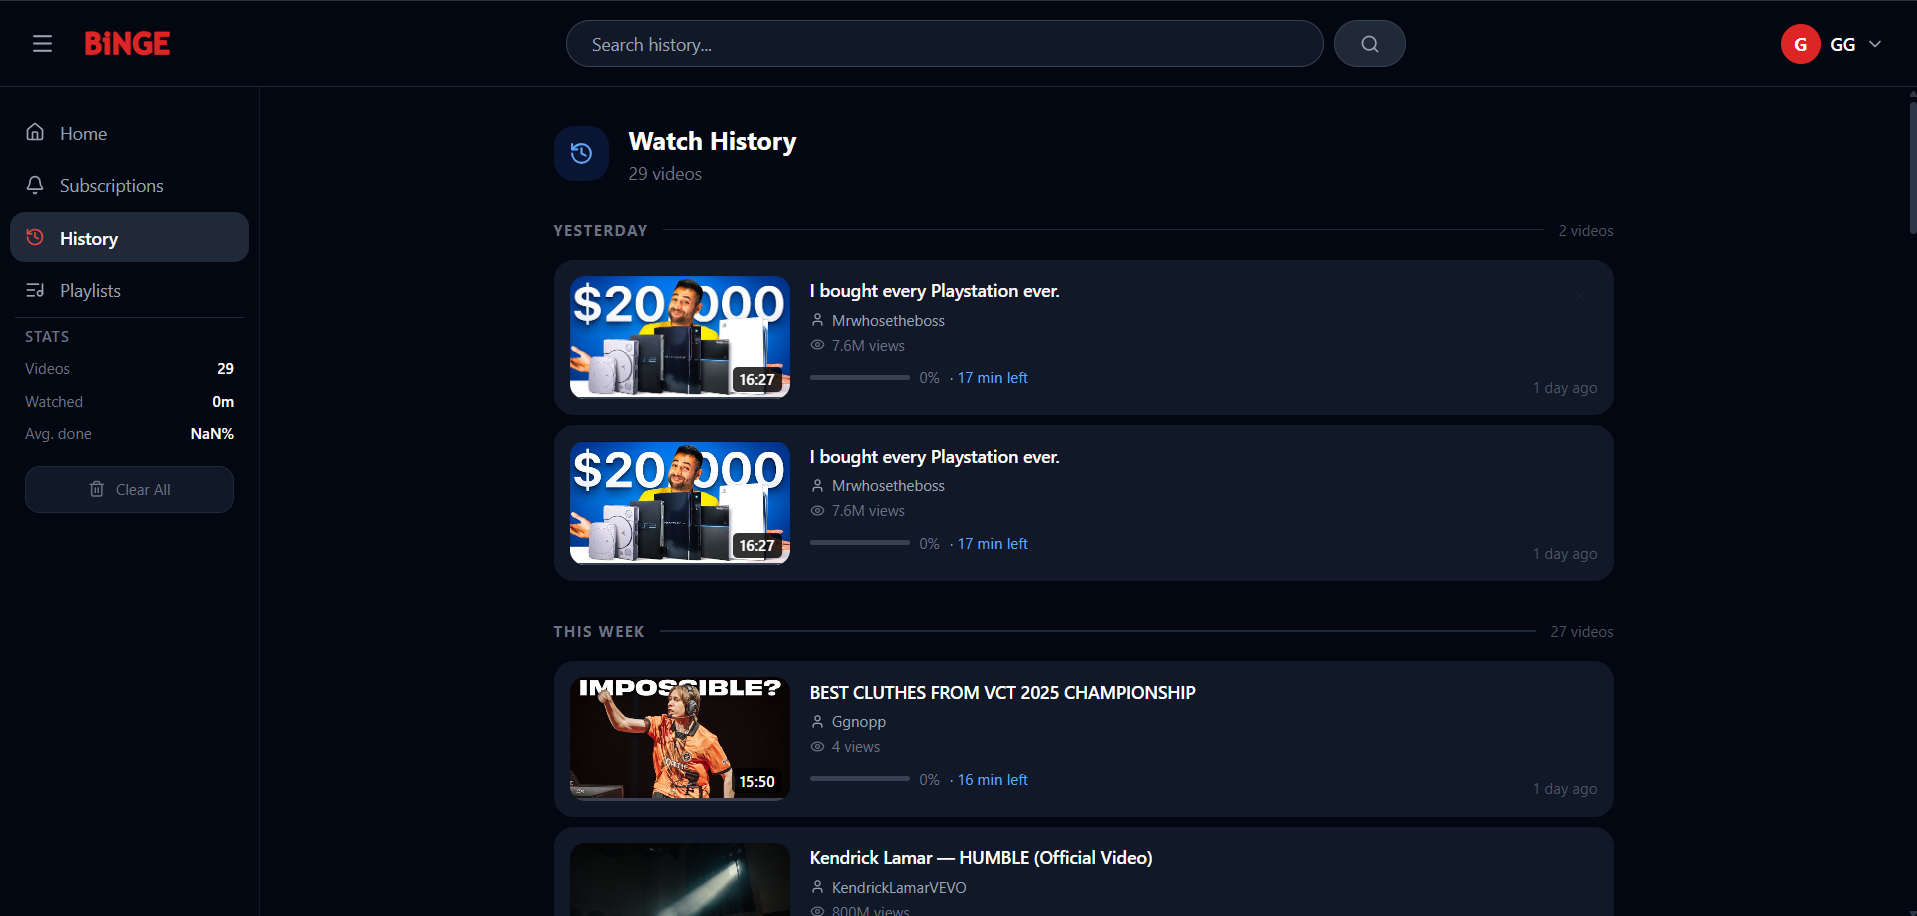
\includegraphics[width=\textwidth,keepaspectratio]{Figures/U05.png}
\caption{U05: Watch History Screen}
\label{fig:U05}
\end{figure}
\clearpage

% ------- U06 -------
\subsection{Manage Playlists}
\begin{table}[ht!]
\centering
\caption{U06: Manage Playlists}
\label{tab:U06}
\begin{tabular}{|>{\hspace{0pt}}m{0.122\linewidth}|>{\hspace{0pt}}m{0.839\linewidth}|}
\hline
Use Case ID & U06 \\ \hline
Name        & Manage Playlists \\ \hline
Actor       & Viewer \\ \hline
Description & The playlists page lists all playlists owned by the viewer with their video count and cover thumbnail (taken from the first video in the playlist). The viewer can create a new playlist by entering a title, description, and visibility (Public / Private / Unlisted). Inside a playlist detail page the viewer can see all videos in order and remove individual ones. Playlist items are stored in the \texttt{playlistitem} table with an \texttt{OrderNo} column that controls the display order. \\ \hline
\end{tabular}
\end{table}

\begin{figure}[ht!]
\centering
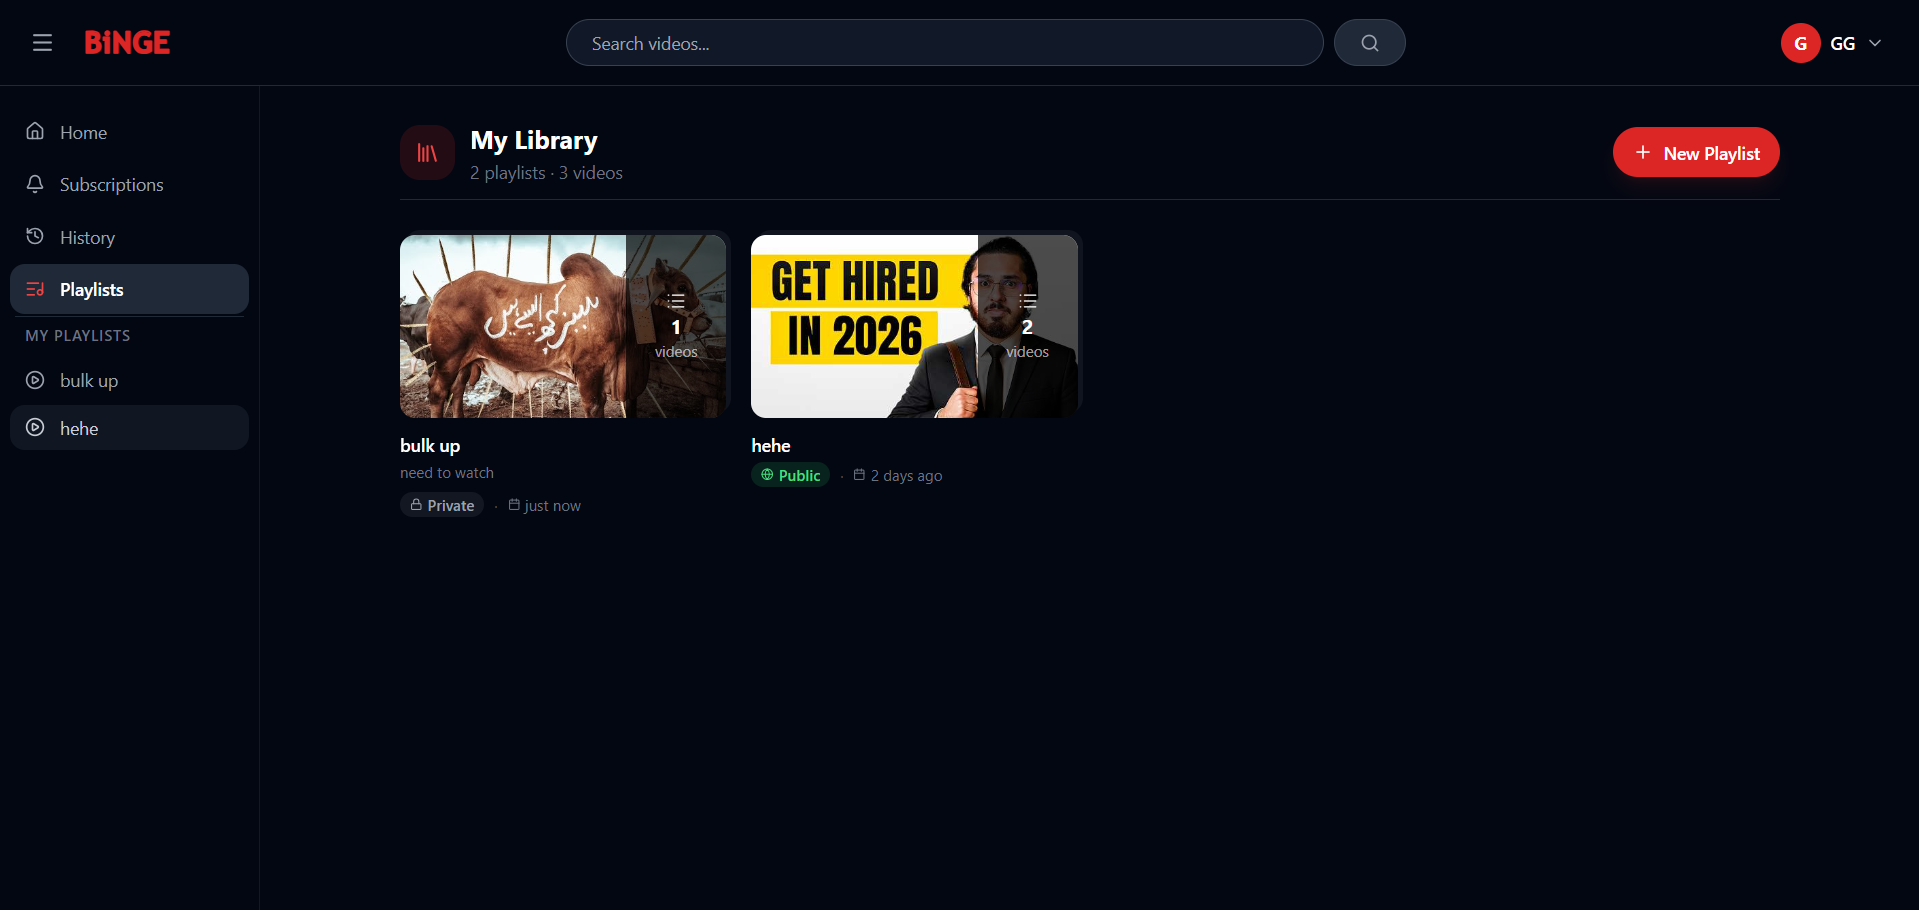
\includegraphics[width=\textwidth,keepaspectratio]{Figures/U06.png}
\caption{U06: Playlists Screen}
\label{fig:U06}
\end{figure}
\clearpage

% ------- U07 -------
\subsection{Subscriptions Feed}
\begin{table}[ht!]
\centering
\caption{U07: Subscriptions Feed}
\label{tab:U07}
\begin{tabular}{|>{\hspace{0pt}}m{0.122\linewidth}|>{\hspace{0pt}}m{0.839\linewidth}|}
\hline
Use Case ID & U07 \\ \hline
Name        & Subscriptions Feed \\ \hline
Actor       & Viewer \\ \hline
Description & The subscriptions page displays two sections: a grid of all channels the viewer is subscribed to (showing subscriber count, total videos, and subscription date), and a chronological feed of the latest videos from those channels. The viewer can also unsubscribe directly from any channel card on this page. \\ \hline
\end{tabular}
\end{table}

\begin{figure}[ht!]
\centering
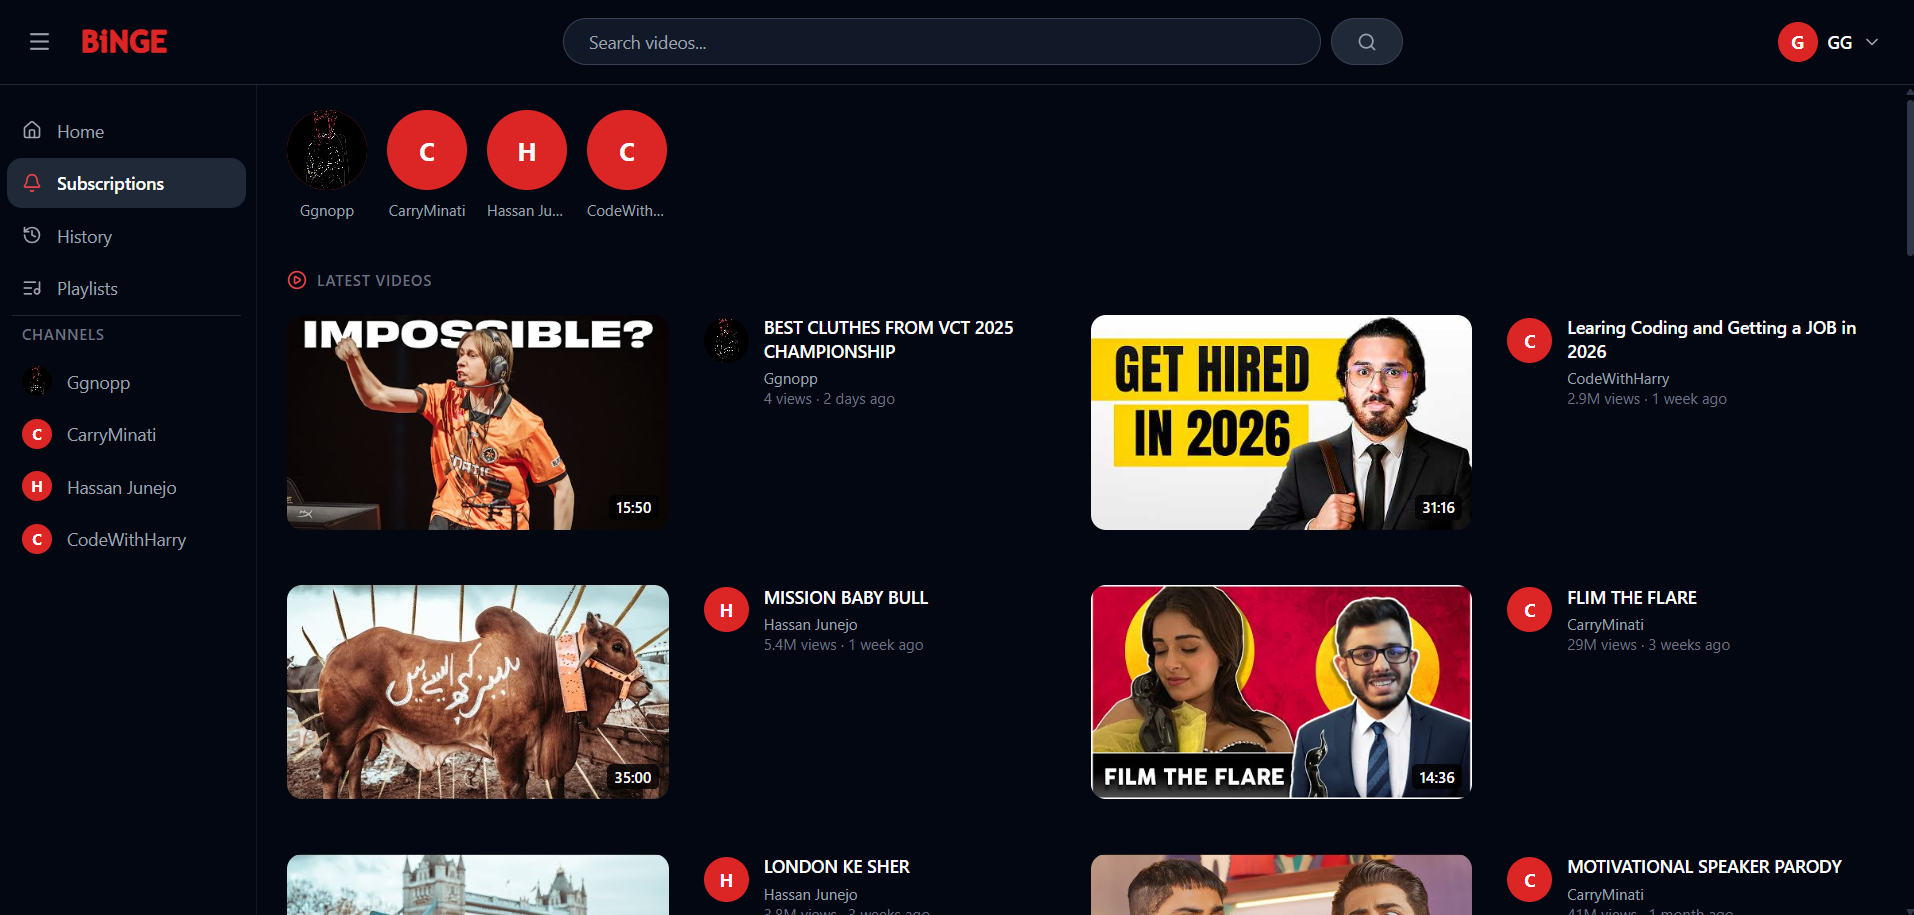
\includegraphics[width=\textwidth,keepaspectratio]{Figures/U07.png}
\caption{U07: Subscriptions Feed Screen}
\label{fig:U07}
\end{figure}
\clearpage

% ------- U08 -------
\subsection{Creator Dashboard}
\begin{table}[ht!]
\centering
\caption{U08: Creator Dashboard}
\label{tab:U08}
\begin{tabular}{|>{\hspace{0pt}}m{0.122\linewidth}|>{\hspace{0pt}}m{0.839\linewidth}|}
\hline
Use Case ID & U08 \\ \hline
Name        & Creator Dashboard \\ \hline
Actor       & Creator \\ \hline
Description & The creator studio shows a header with the channel name, subscriber count, and bio. Four stat cards display total videos, total views, total subscribers, and total likes. These figures are fetched by querying the \texttt{vw\_CreatorDashboard} view — the same view that powers the admin Creators tab — filtered by the logged-in creator's ID. Below the stats, a table lists all of the creator's videos with their view count, status badge, and Edit / Delete action buttons. \\ \hline
\end{tabular}
\end{table}

\begin{figure}[ht!]
\centering
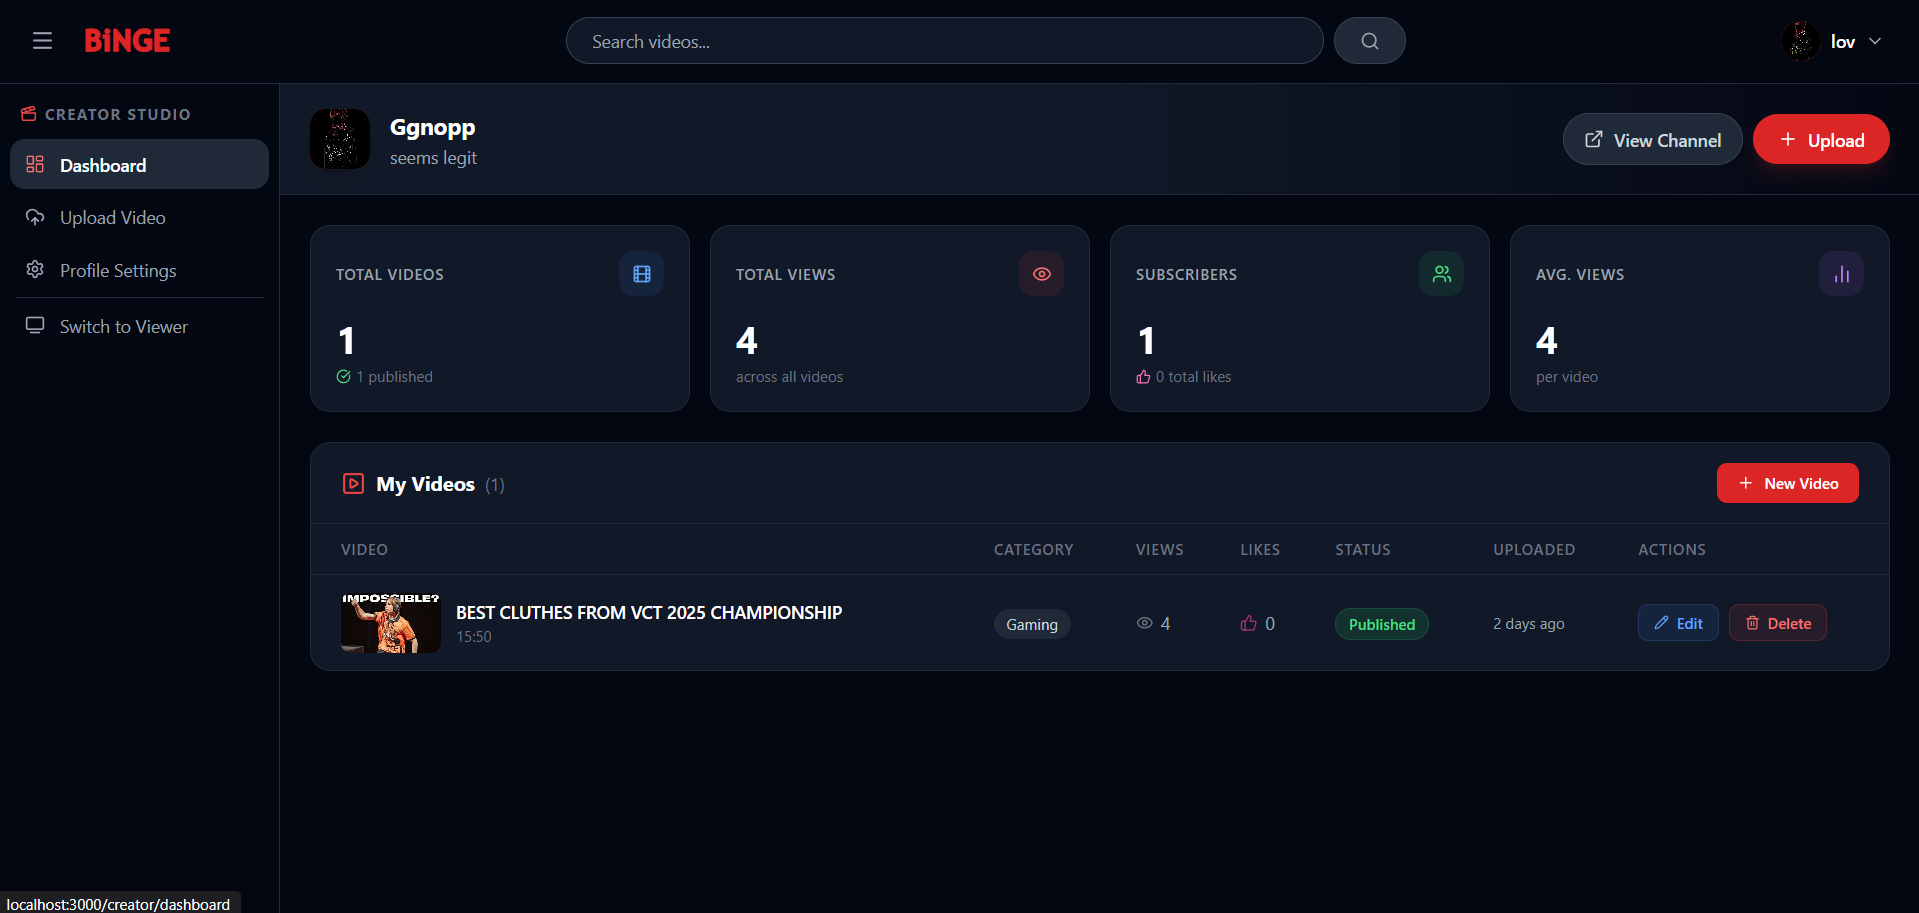
\includegraphics[width=\textwidth,keepaspectratio]{Figures/U08.png}
\caption{U08: Creator Dashboard Screen}
\label{fig:U08}
\end{figure}
\clearpage

% ------- U09 -------
\subsection{Upload Video}
\begin{table}[ht!]
\centering
\caption{U09: Upload Video}
\label{tab:U09}
\begin{tabular}{|>{\hspace{0pt}}m{0.122\linewidth}|>{\hspace{0pt}}m{0.839\linewidth}|}
\hline
Use Case ID & U09 \\ \hline
Name        & Upload Video \\ \hline
Actor       & Creator \\ \hline
Description & The creator fills in the title, description, YouTube video URL, duration (seconds), category, publish status (Published / Private / Draft), and one or more tags. Input is validated by the \texttt{Validator} class. On submission the stored procedure \texttt{sp\_UploadVideo} is called which atomically inserts the video row inside a transaction and returns the new video ID via an OUT parameter. Tag associations are then inserted into the \texttt{videotag} table. The \texttt{trg\_AfterVideoPublished} trigger fires automatically and inserts notifications for all subscribers. \\ \hline
\end{tabular}
\end{table}

\begin{figure}[ht!]
\centering
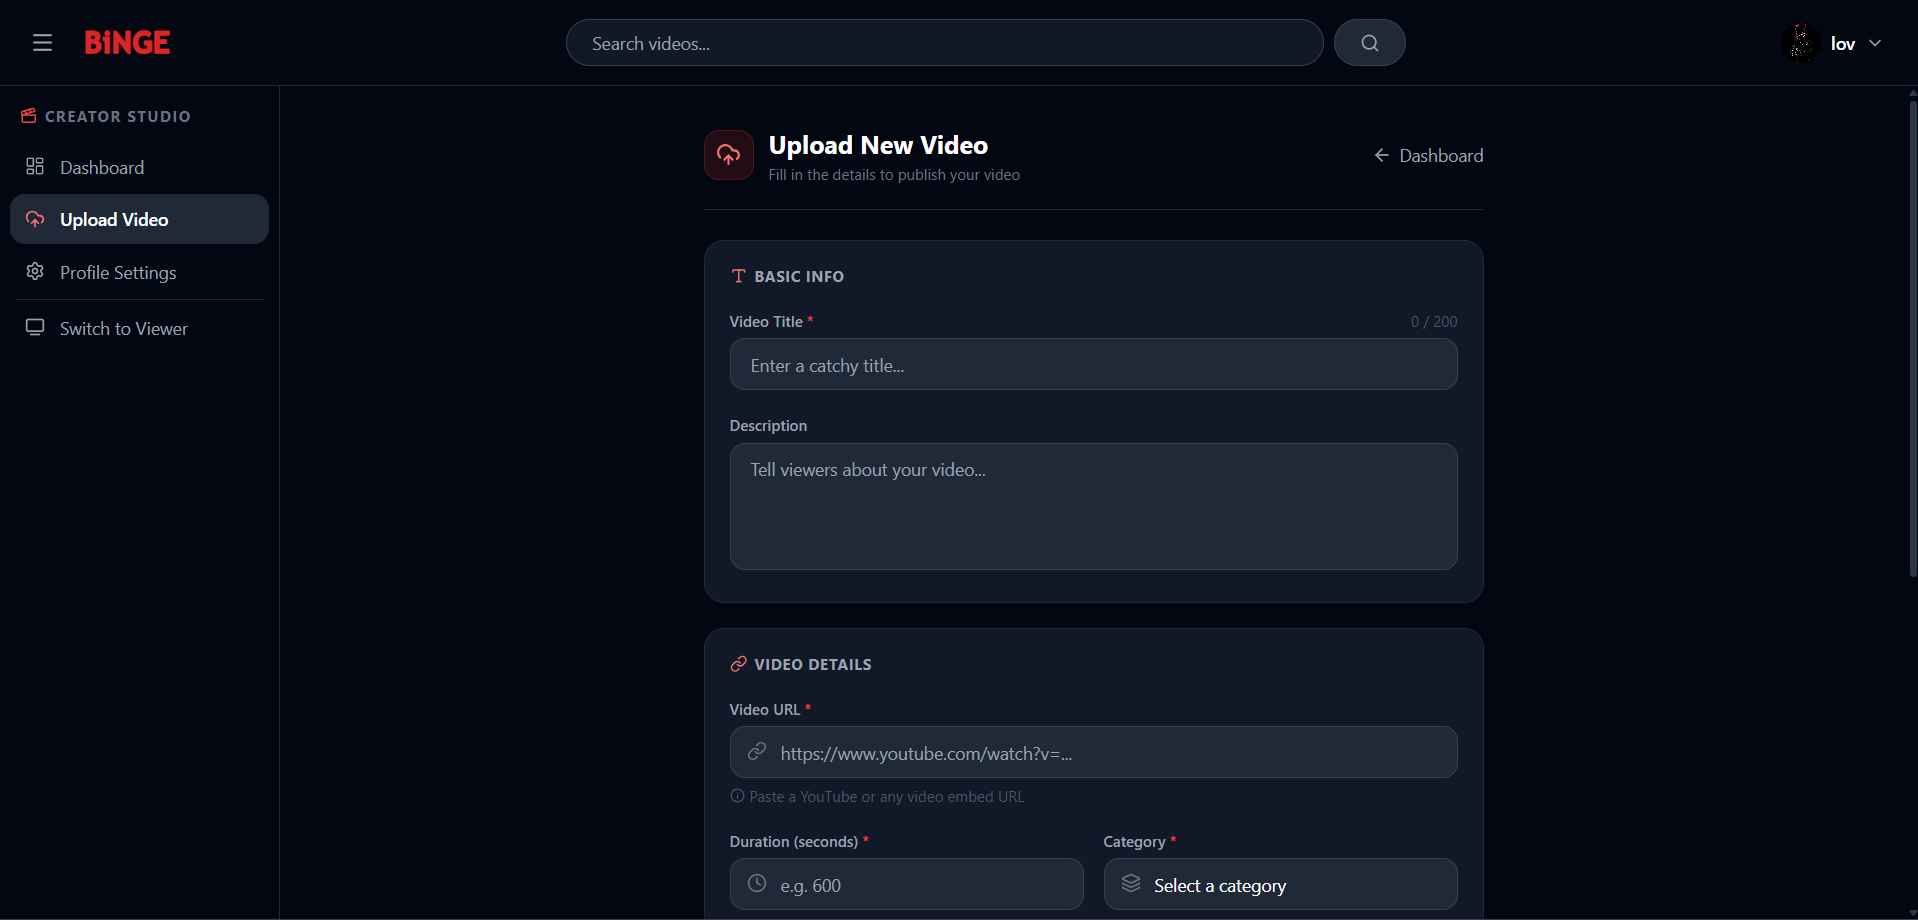
\includegraphics[width=\textwidth,keepaspectratio]{Figures/U09.png}
\caption{U09: Upload Video Screen}
\label{fig:U09}
\end{figure}
\clearpage

% ------- U10 -------
\subsection{Edit / Delete Video}
\begin{table}[ht!]
\centering
\caption{U10: Edit / Delete Video}
\label{tab:U10}
\begin{tabular}{|>{\hspace{0pt}}m{0.122\linewidth}|>{\hspace{0pt}}m{0.839\linewidth}|}
\hline
Use Case ID & U10 \\ \hline
Name        & Edit / Delete Video \\ \hline
Actor       & Creator \\ \hline
Description & From the dashboard video table the creator can edit or delete any of their videos. \textbf{Edit:} the upload form re-opens pre-filled with existing values. On submission a database transaction is opened: the \texttt{video} row is updated, all existing \texttt{videotag} rows for that video are deleted, and the new selection is re-inserted. If any step fails the whole transaction is rolled back. \textbf{Delete:} the video is removed from the database; the \texttt{trg\_AfterVideoDelete} trigger fires and recalculates the creator's \texttt{TotalViews}. \\ \hline
\end{tabular}
\end{table}

\begin{figure}[ht!]
\centering
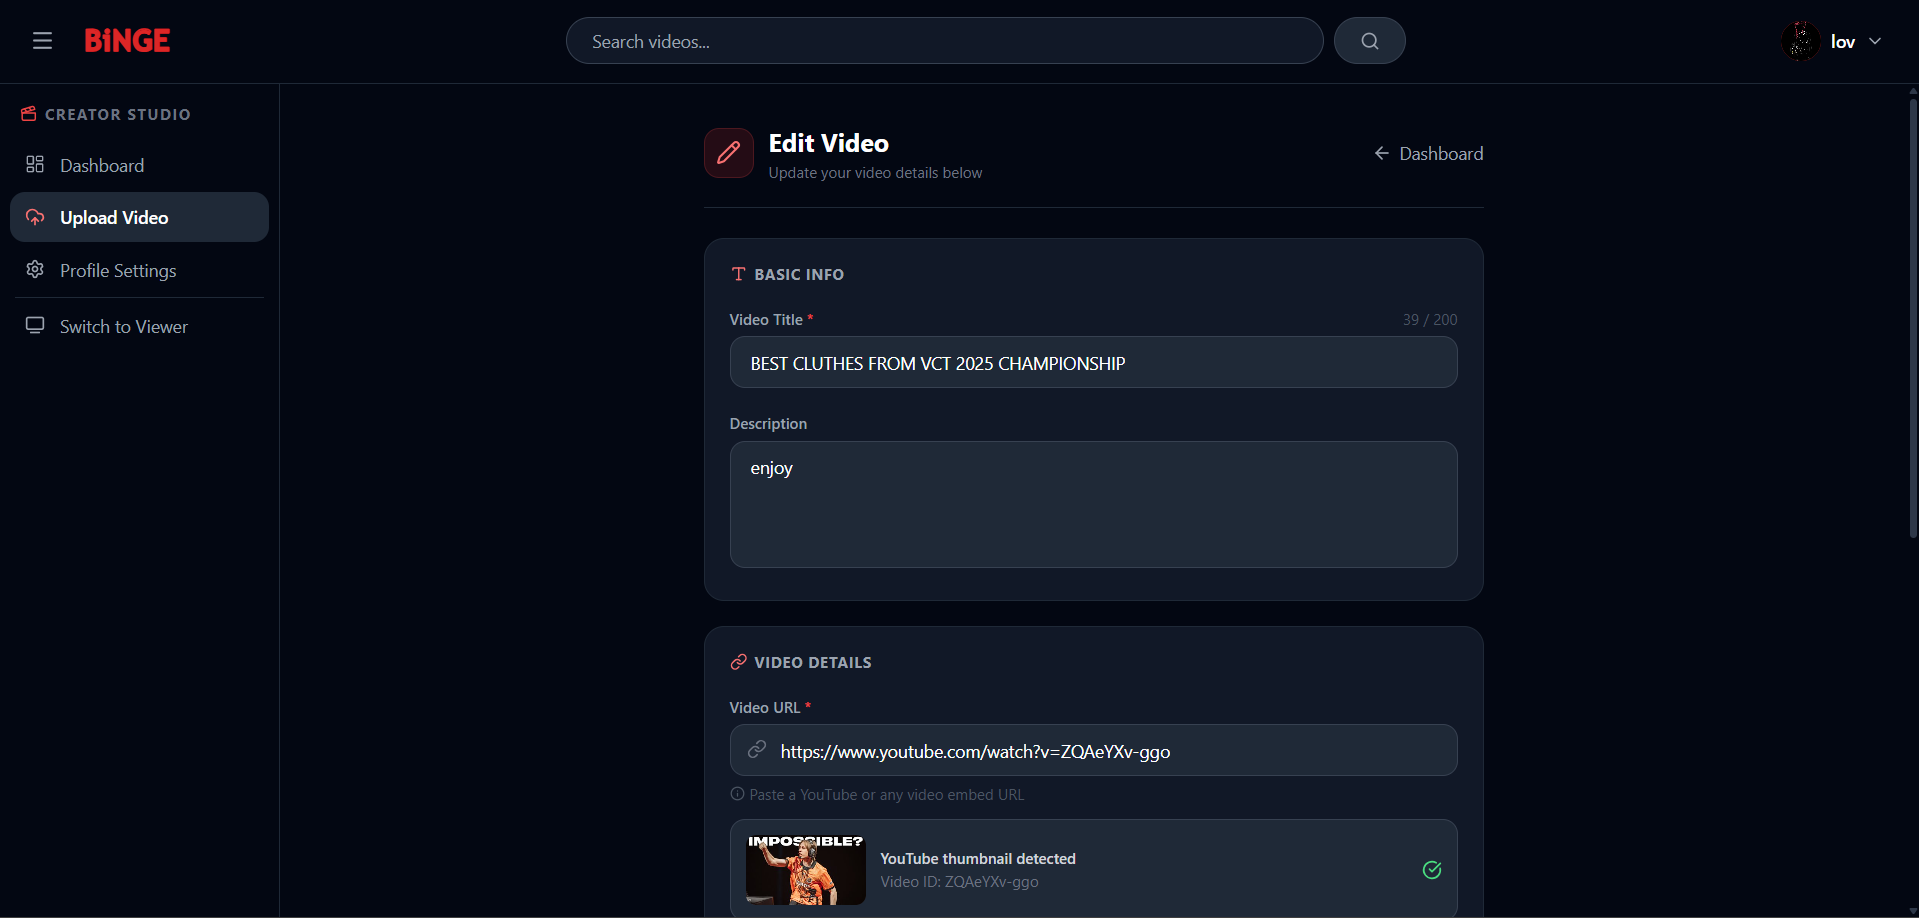
\includegraphics[width=\textwidth,keepaspectratio]{Figures/U10.png}
\caption{U10: Edit Video Screen}
\label{fig:U10}
\end{figure}
\clearpage

% ------- U11 -------
\subsection{Creator Profile}
\begin{table}[ht!]
\centering
\caption{U11: Creator Profile}
\label{tab:U11}
\begin{tabular}{|>{\hspace{0pt}}m{0.122\linewidth}|>{\hspace{0pt}}m{0.839\linewidth}|}
\hline
Use Case ID & U11 \\ \hline
Name        & Creator Profile \\ \hline
Actor       & Creator \\ \hline
Description & The creator profile page allows the creator to update their personal information (first name, last name, country), channel information (channel name, bio), and profile avatar. The avatar is uploaded using Multer which saves the file to the \texttt{public/uploads} directory and stores the filename in the \texttt{user.Avatar} column. The session is updated immediately so the navbar reflects the new avatar without requiring a re-login. \\ \hline
\end{tabular}
\end{table}

\begin{figure}[ht!]
\centering
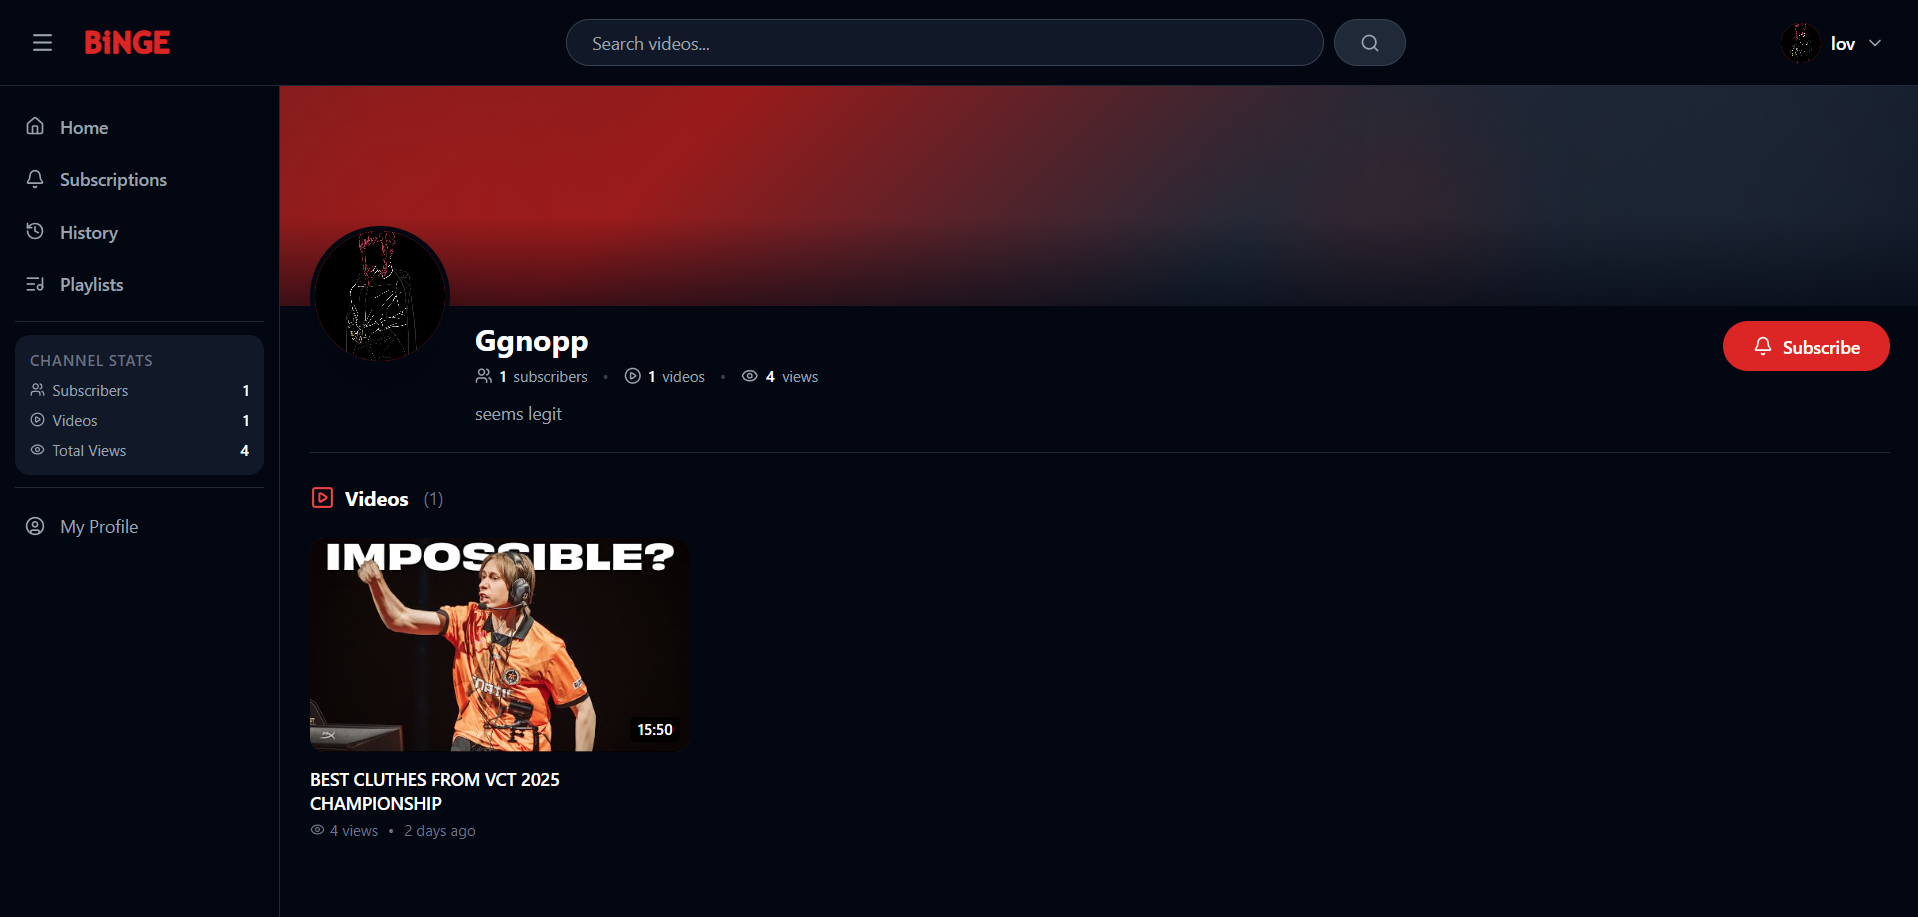
\includegraphics[width=\textwidth,keepaspectratio]{Figures/U11.png}
\caption{U11: Creator Profile Screen}
\label{fig:U11}
\end{figure}
\clearpage

% ------- U12 -------
\subsection{Admin Dashboard}
\begin{table}[ht!]
\centering
\caption{U12: Admin Dashboard}
\label{tab:U12}
\begin{tabular}{|>{\hspace{0pt}}m{0.122\linewidth}|>{\hspace{0pt}}m{0.839\linewidth}|}
\hline
Use Case ID & U12 \\ \hline
Name        & Admin Dashboard \\ \hline
Actor       & Admin \\ \hline
Description & The admin dashboard displays six platform-wide stat cards (total users, videos, creators, comments, views, and pending reports). Below it a tabbed interface provides four tabs: \textbf{Users} -- lists all registered users with role badges and suspend/activate buttons; \textbf{Videos} -- lists all videos with delete action; \textbf{Creators} -- shows a table powered by the \texttt{vw\_CreatorDashboard} view with per-channel stats (subscribers, views, videos, likes, comments); \textbf{Moderation} -- shows pending reports with dismiss and action buttons. \\ \hline
\end{tabular}
\end{table}

\begin{figure}[ht!]
\centering
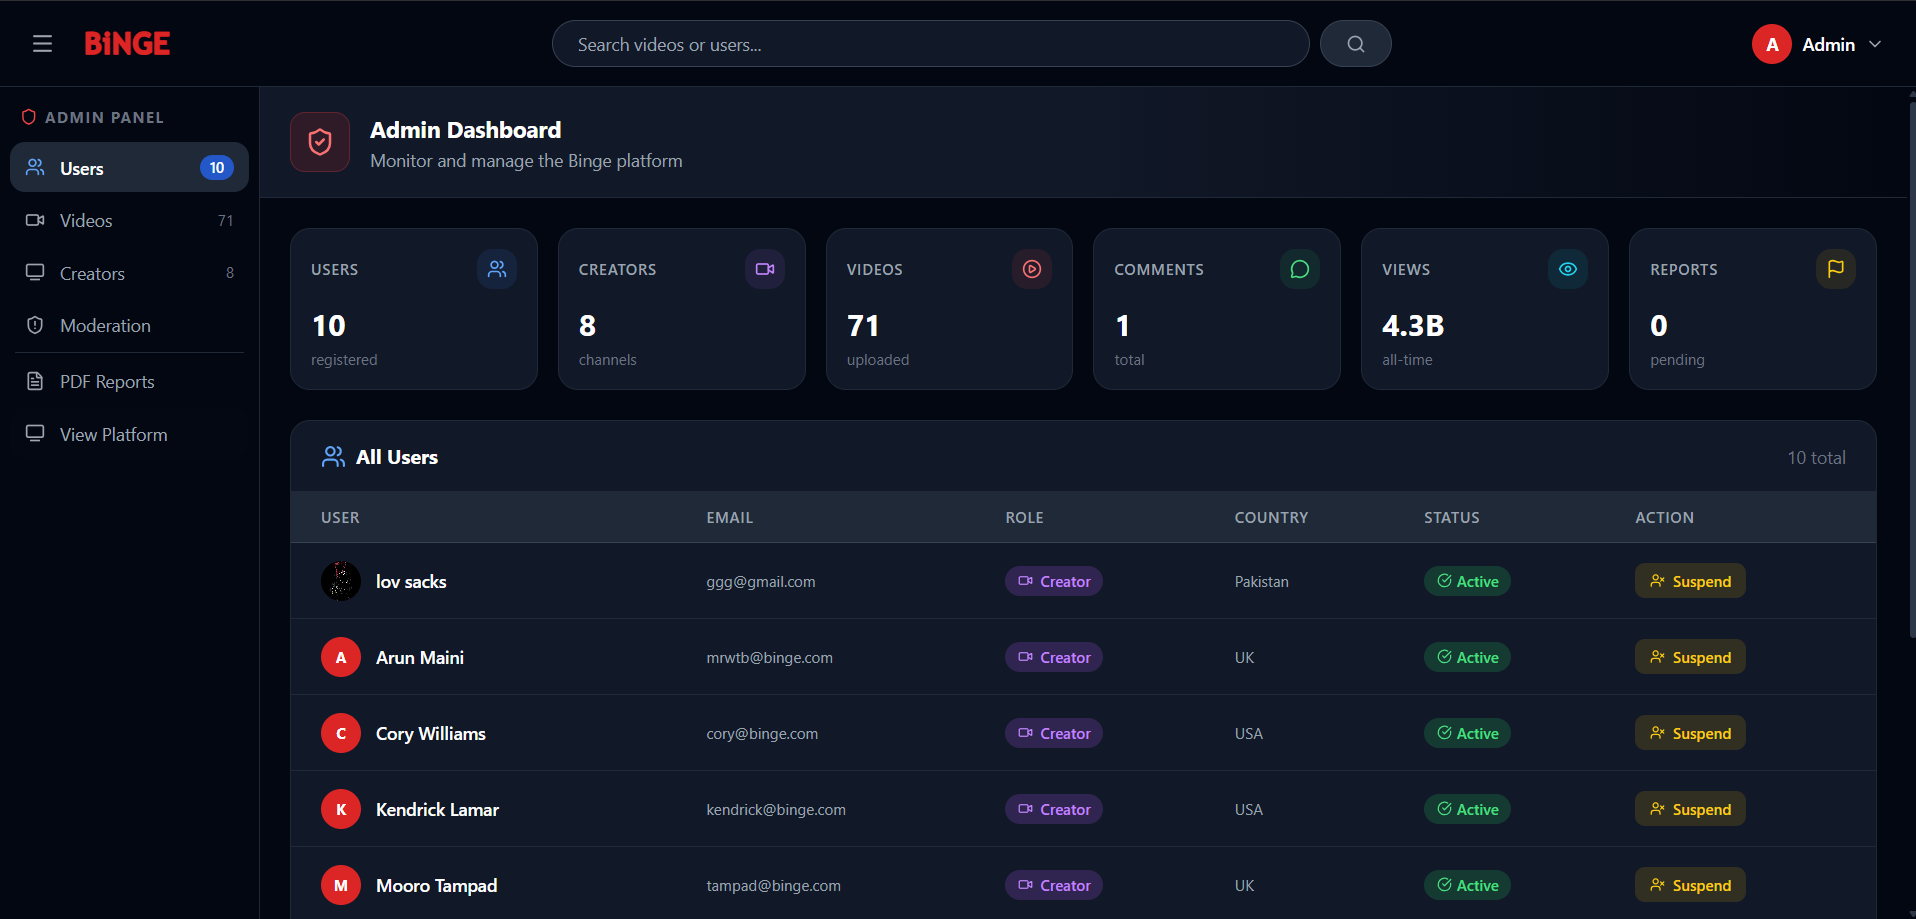
\includegraphics[width=\textwidth,keepaspectratio]{Figures/U12.png}
\caption{U12: Admin Dashboard Screen}
\label{fig:U12}
\end{figure}
\clearpage

% ------- U13 -------
\subsection{Generate PDF Reports}
\begin{table}[ht!]
\centering
\caption{U13: Generate PDF Reports}
\label{tab:U13}
\begin{tabular}{|>{\hspace{0pt}}m{0.122\linewidth}|>{\hspace{0pt}}m{0.839\linewidth}|}
\hline
Use Case ID & U13 \\ \hline
Name        & Generate PDF Reports \\ \hline
Actor       & Admin \\ \hline
Description & The admin reports page lists 10 available reports. Each report has optional filter inputs (e.g., date range, category, country, status). Clicking the generate button sends a request to the server which executes a database query (often against a view), builds a PDF document using PDFKit, and streams it directly to the browser. Reports include trending videos, creator stats, category engagement, user activity, monthly watch summary, and more. \\ \hline
\end{tabular}
\end{table}

\begin{figure}[ht!]
\centering
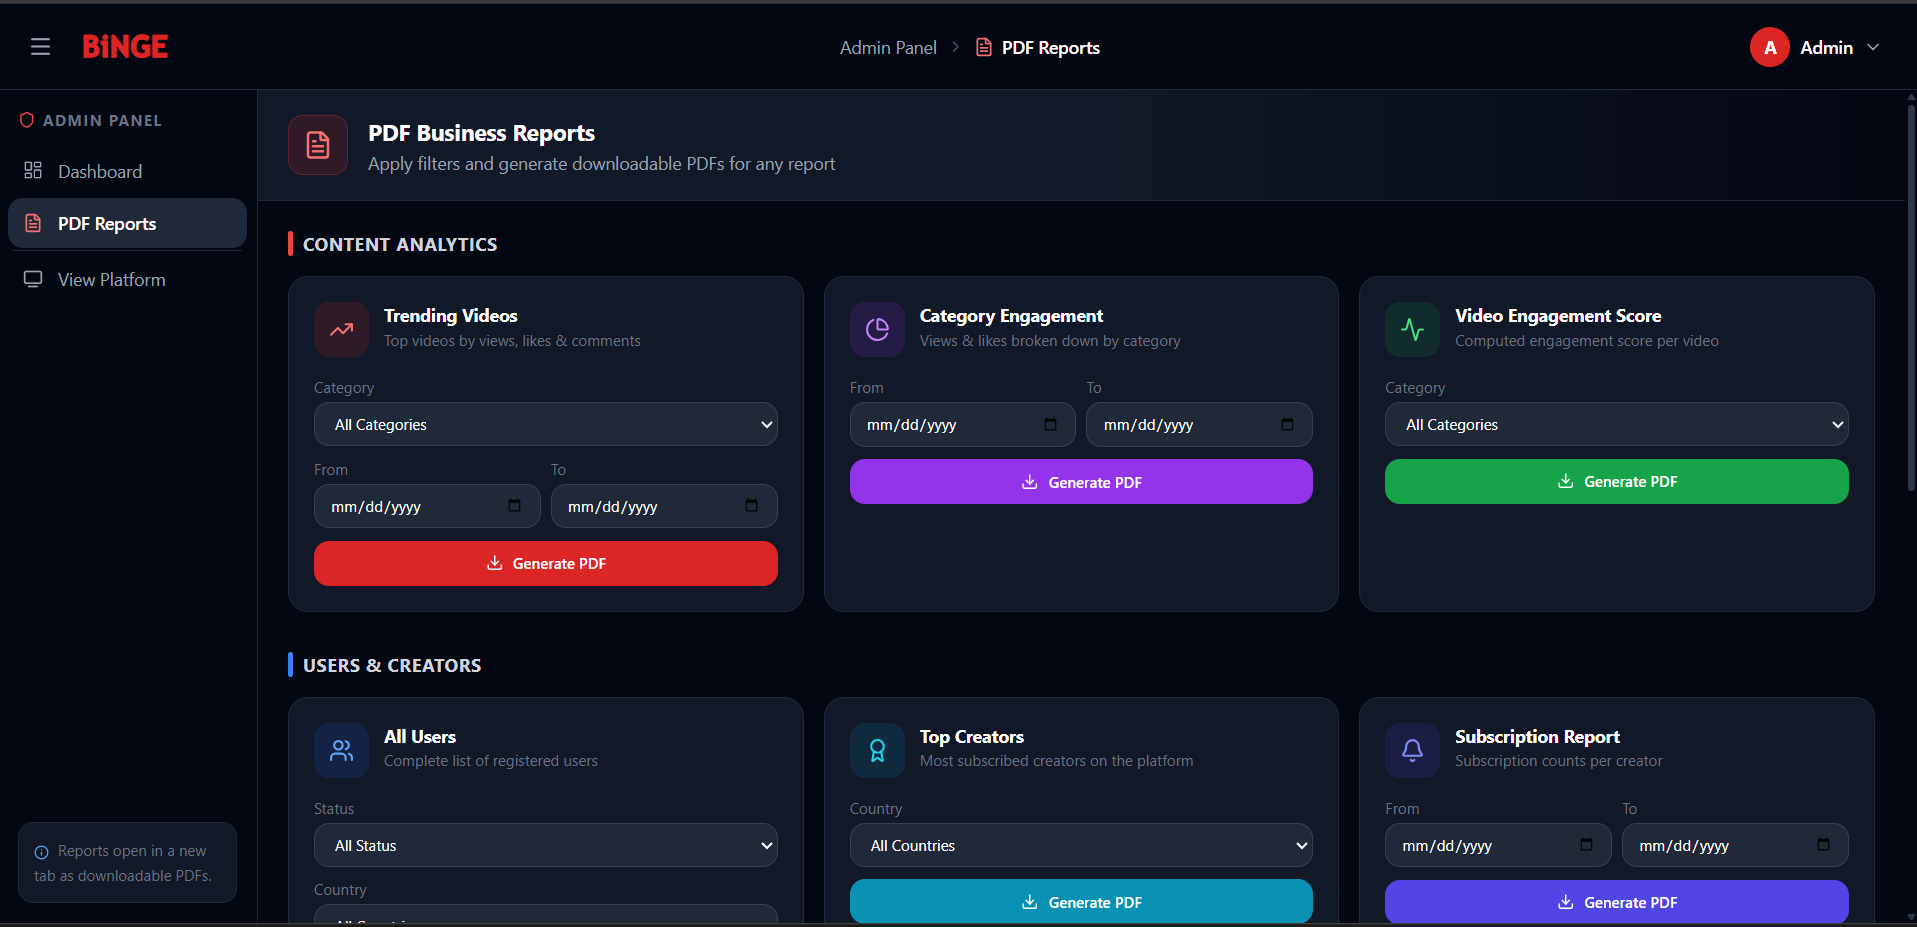
\includegraphics[width=\textwidth,keepaspectratio]{Figures/U13.png}
\caption{U13: PDF Reports Page}
\label{fig:U13}
\end{figure}
\clearpage

% ============================================================
\section{PDF Generation Methodology}
% ============================================================

PDFKit is a Node.js PDF generation library that allows creating PDF documents programmatically and streaming them directly in an HTTP response. This package is used in this project to generate all 10 admin reports on demand.

A new PDF document is created with A4 size and 40pt margins as follows:

\begin{lstlisting}[language=JavaScript, caption={Creating a PDFDocument}]
const doc = new PDFDocument({ margin: 40, size: 'A4' });
res.setHeader('Content-Type', 'application/pdf');
res.setHeader('Content-Disposition', 'inline; filename="report.pdf"');
doc.pipe(res);
\end{lstlisting}

The \texttt{pipe(res)} call streams the PDF bytes directly to the HTTP response, meaning no file is saved on the server. The report header is drawn using colored rectangles and text:

\begin{lstlisting}[language=JavaScript, caption={Drawing the page header}]
doc.fillColor('#CC0000').fontSize(22).font('Helvetica-Bold').text('Binge', 40, 40);
doc.fillColor('#333').fontSize(14).font('Helvetica-Bold').text(title, 40, 68);
doc.moveTo(40, 105).lineTo(doc.page.width - 40, 105)
   .strokeColor('#CC0000').lineWidth(1.5).stroke();
\end{lstlisting}

A data table is drawn by calculating column widths proportionally and iterating over the rows. Alternating row colours are applied for readability:

\begin{lstlisting}[language=JavaScript, caption={Drawing a table row}]
const fill = ri % 2 === 0 ? '#f9f9f9' : 'white';
doc.fillColor(fill).rect(40, y, doc.page.width - 80, rowHeight).fill();
doc.fillColor('#333333').fontSize(8).font('Helvetica');
row.forEach((cell, i) => {
    doc.text(String(cell ?? '-'), 40 + i * colWidth + 5, y + 7,
             { width: colWidth - 10 });
});
\end{lstlisting}

When the content reaches the bottom of the page a new page is added automatically:

\begin{lstlisting}[language=JavaScript, caption={Automatic page break}]
if (y > doc.page.height - 80) {
    doc.addPage();
    y = 50;
}
\end{lstlisting}

Finally the document is closed to flush and end the stream:

\begin{lstlisting}[language=JavaScript, caption={Ending the document}]
doc.end();
\end{lstlisting}

% ============================================================
\section{PDF Reports}
% ============================================================

Ten reports are generated using the PDFKit methodology described above. Each report queries the database (often through a view) and renders a formatted table.

\subsection{Trending Videos Report}
Powered by the \texttt{vw\_TrendingVideos} view. Displays the top 20 most-viewed published videos with their channel, category, like count, comment count, and upload date. Optional date range filters are supported.

\begin{figure}[ht!]
\centering
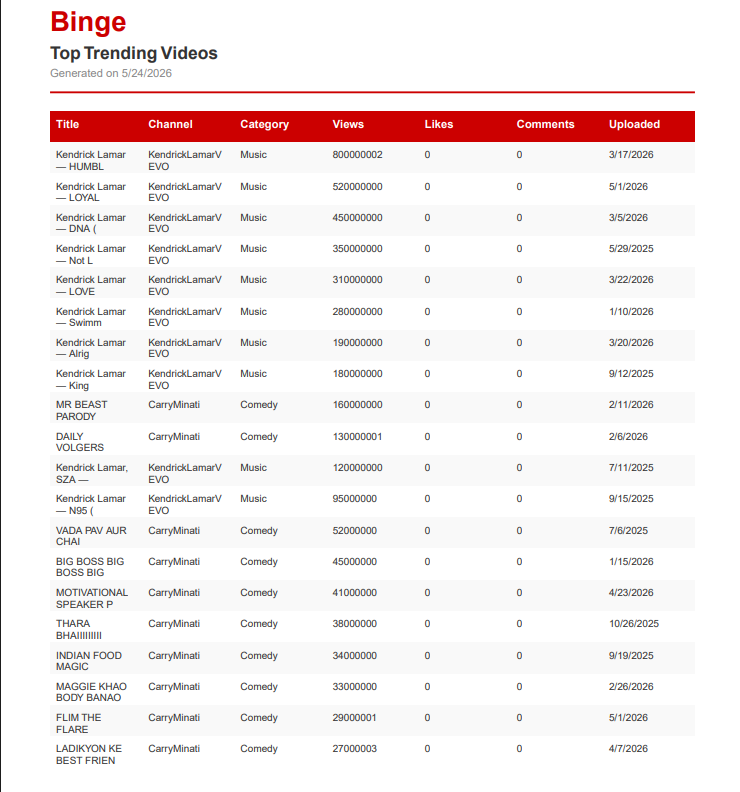
\includegraphics[width=\textwidth,keepaspectratio]{Figures/R01.png}
\caption{Trending Videos PDF Report}
\label{fig:R01}
\end{figure}
\clearpage

\subsection{Creator Stats Report}
Powered by the \texttt{vw\_CreatorStats} view. Lists all creators with their active subscriber count, published video count, real total views, estimated revenue, and country. Can be filtered by country.

\begin{figure}[ht!]
\centering
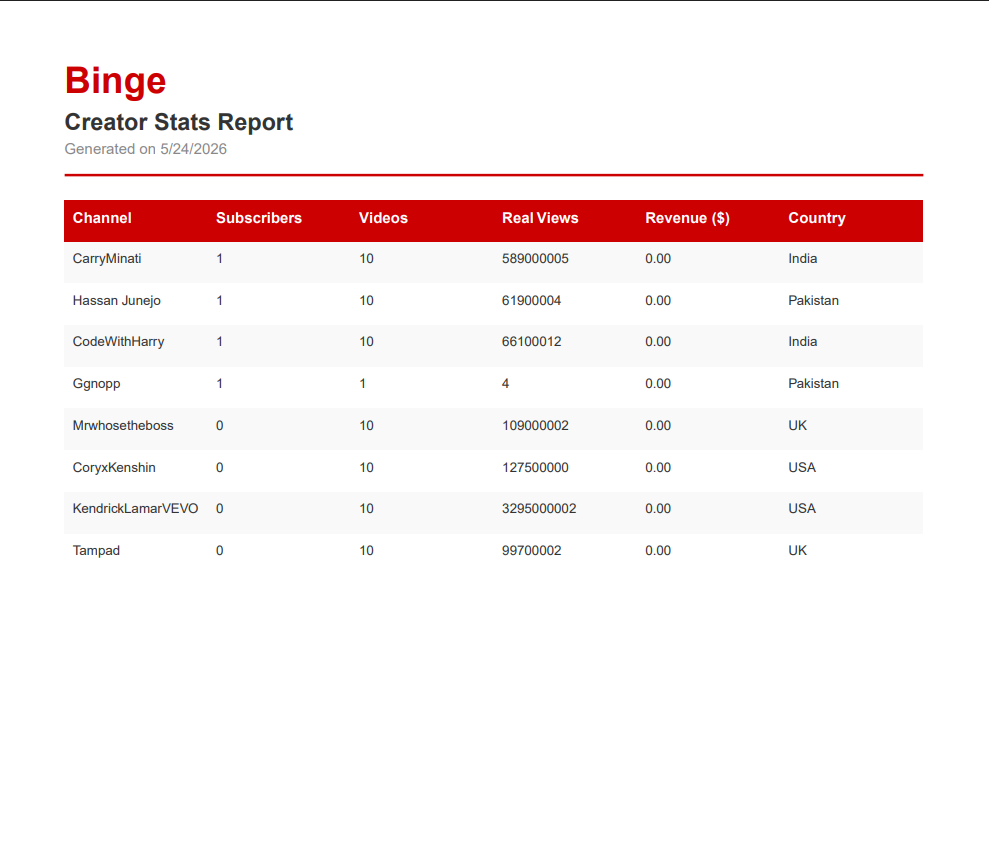
\includegraphics[width=\textwidth,keepaspectratio]{Figures/R02.png}
\caption{Creator Stats PDF Report}
\label{fig:R02}
\end{figure}
\clearpage

\subsection{Category Engagement Report}
Powered by the \texttt{vw\_TopCategories} view. Shows every category with total video count, total views, and total likes across the platform.

\begin{figure}[ht!]
\centering
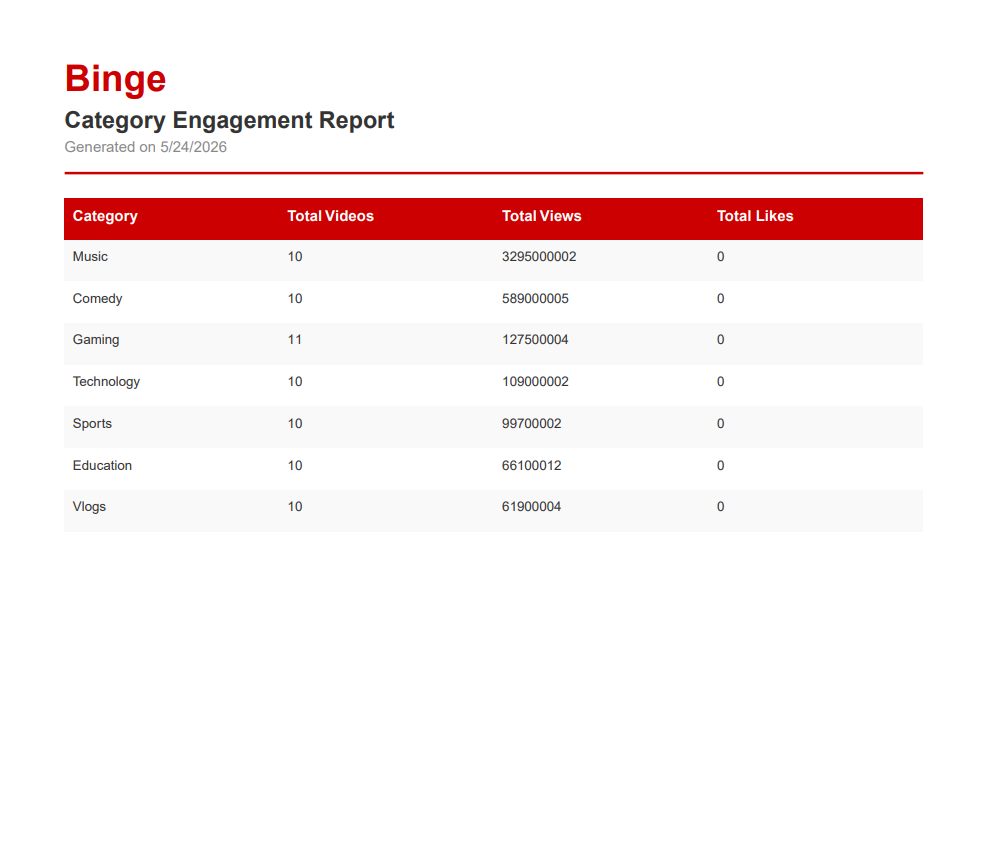
\includegraphics[width=\textwidth,keepaspectratio]{Figures/R03.png}
\caption{Category Engagement PDF Report}
\label{fig:R03}
\end{figure}

\subsection{Video Engagement Score Report}
Powered by the \texttt{vw\_VideoEngagement} view. Shows each video's engagement score calculated as: $(Views \times 0.5) + (Likes \times 2) + (Comments \times 3)$, along with average completion percentage.

\begin{figure}[ht!]
\centering
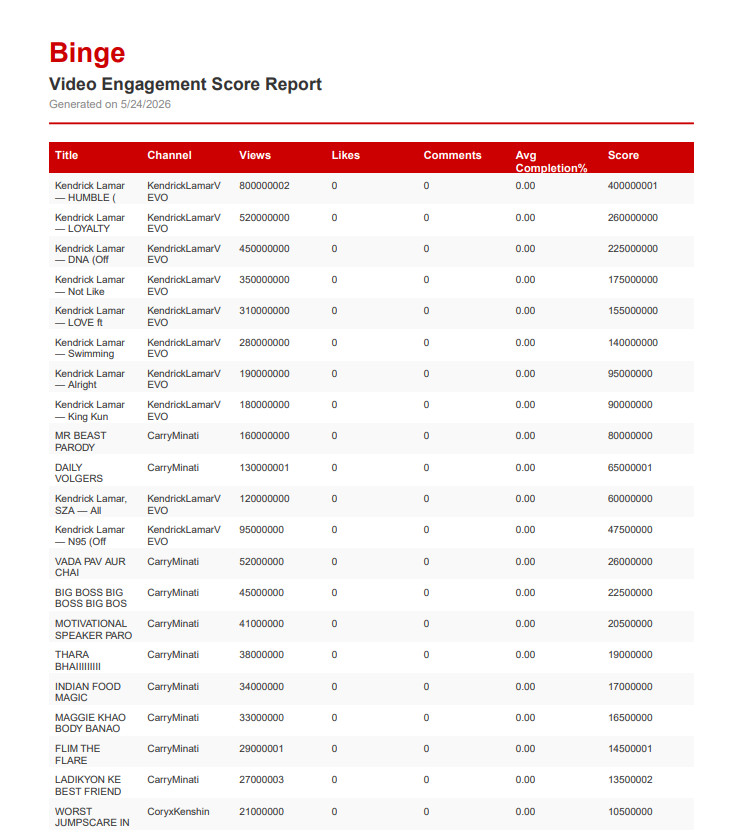
\includegraphics[width=\textwidth,keepaspectratio]{Figures/R04.png}
\caption{Video Engagement Score PDF Report}
\label{fig:R04}
\end{figure}
\clearpage

\subsection{Monthly Watch Summary Report}
Powered by the \texttt{vw\_MonthlyWatchSummary} view. Provides a month-by-month breakdown of total watches, unique viewers, unique videos watched, and average completion percentage.

\begin{figure}[ht!]
\centering
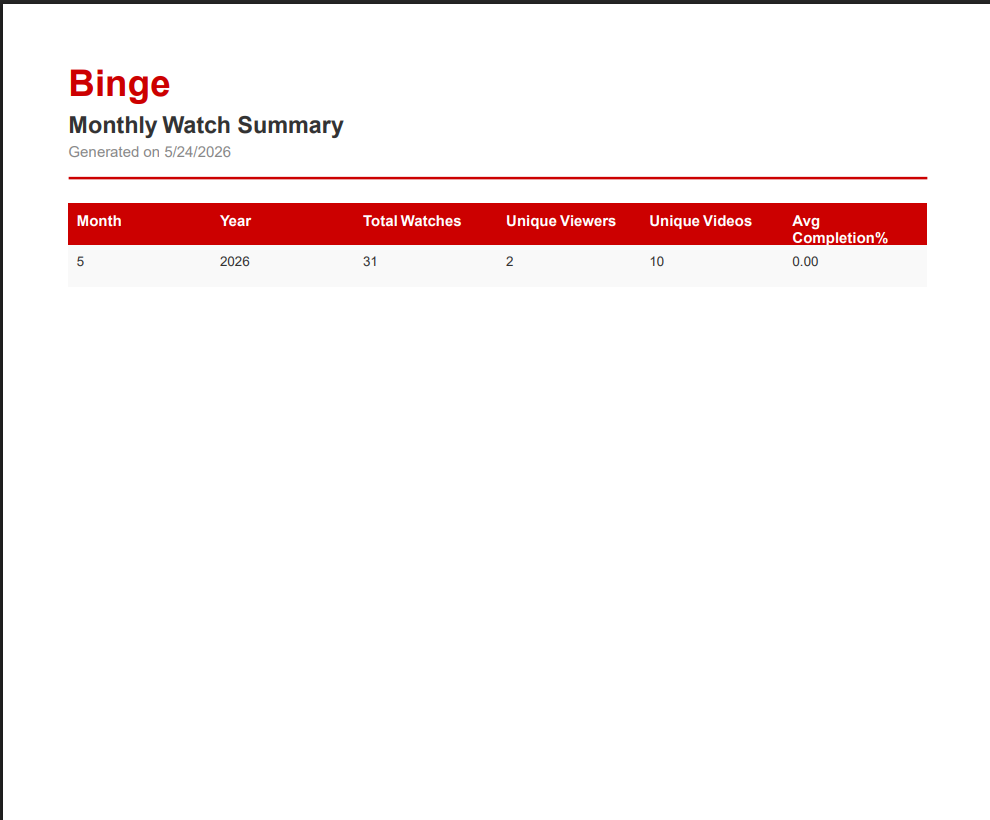
\includegraphics[width=\textwidth,keepaspectratio]{Figures/R05.png}
\caption{Monthly Watch Summary PDF Report}
\label{fig:R05}
\end{figure}

\subsection{User Activity Report}
Powered by the \texttt{vw\_UserActivity} view. Lists all users with their videos watched count, comments made, likes given, subscriptions count, and last active date. Can be filtered by status and country.

\begin{figure}[ht!]
\centering
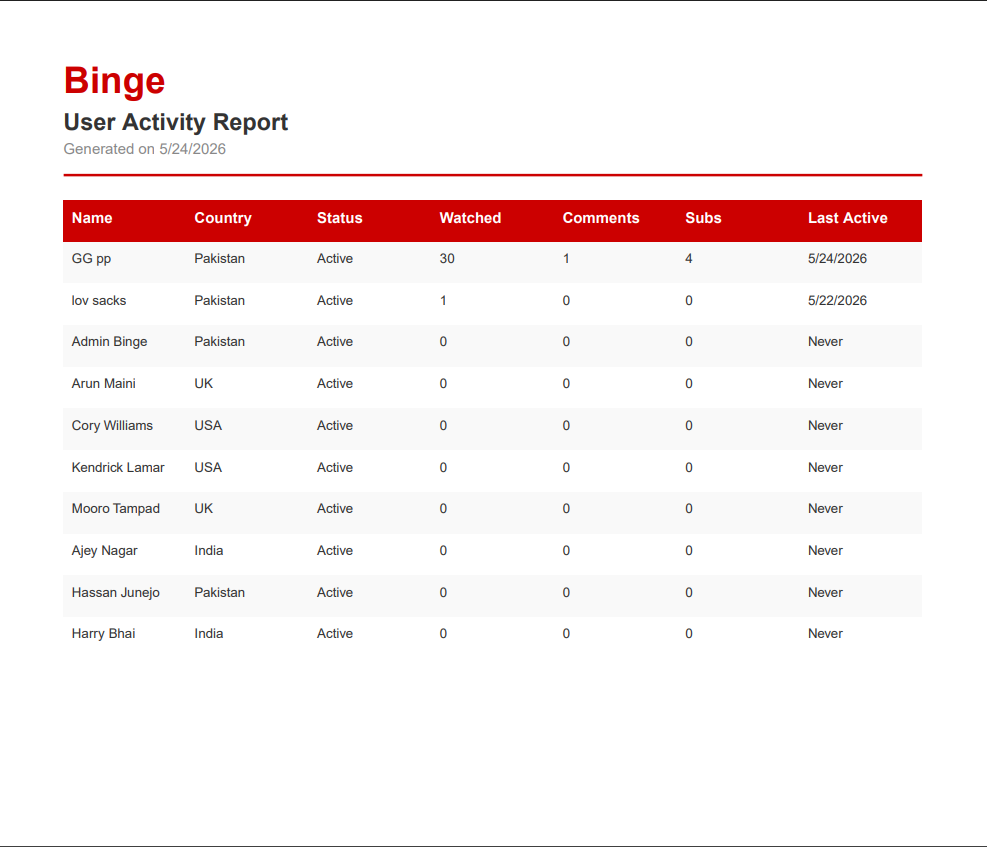
\includegraphics[width=\textwidth,keepaspectratio]{Figures/R06.png}
\caption{User Activity PDF Report}
\label{fig:R06}
\end{figure}
\clearpage

\subsection{All Videos Report}
Custom query with optional status and category filters. Displays video title, channel, category, view count, status, and upload date.

\subsection{Comment Activity Report}
Custom query showing total comment count and last comment date per video, ordered by most commented.

\subsection{Subscription Report}
Custom query showing each creator's channel, total subscribers, active subscription count, and last subscription date.

\subsection{Content Moderation Report}
Custom query with optional status filter showing all reports filed with the video title, reporter name, reason, status, and date reported.

% ============================================================
\section{Database Design}
% ============================================================

\subsection{Entity Relationship Diagram}

\begin{figure}[ht!]
\centering
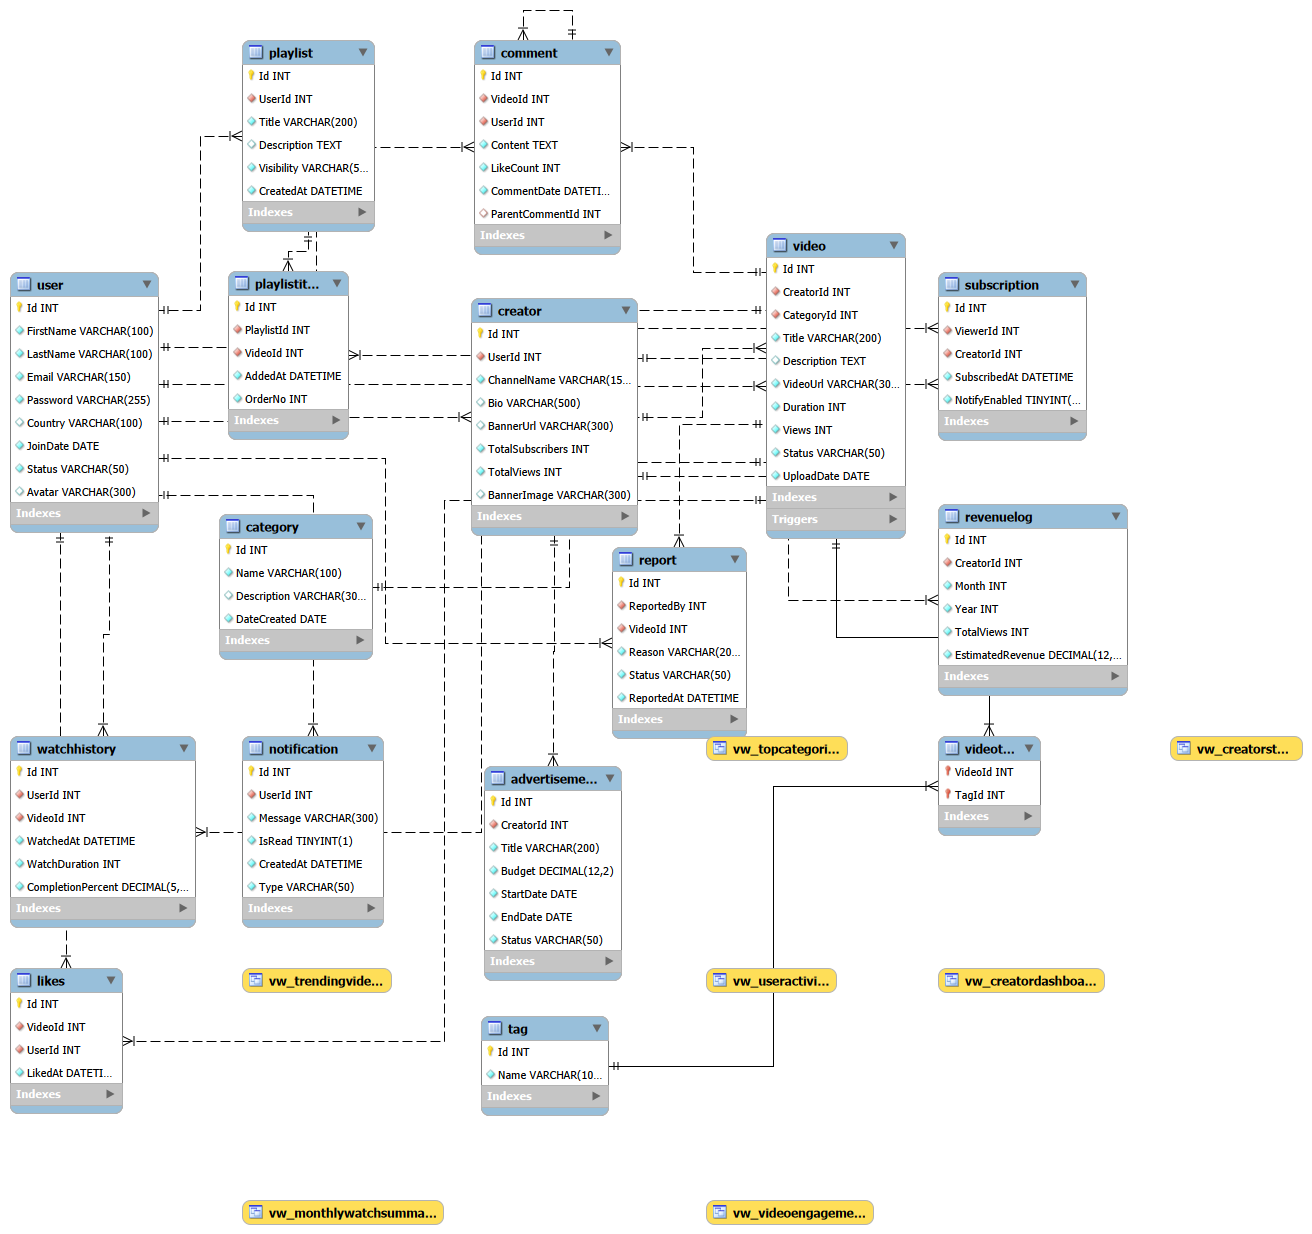
\includegraphics[width=\textwidth,keepaspectratio]{Figures/erd.png}
\caption{Entity Relationship Diagram}
\label{fig:erd}
\end{figure}
\clearpage

\subsection{Tables}

The database contains 16 tables. All primary keys, foreign keys, unique constraints, and check constraints are named for clarity.

\begin{table}[H]
\centering
\caption{Database Tables}
\label{tab:DBTables}
\begin{tabular}{|l|l|l|}
\hline
\textbf{Table}       & \textbf{Key Columns}                                          & \textbf{Purpose}                          \\ \hline
user                 & Id, Email, Password, Status, Avatar                           & Platform user accounts                    \\ \hline
creator              & Id, UserId, ChannelName, TotalSubscribers                     & Creator channel profiles                  \\ \hline
video                & Id, CreatorId, CategoryId, Title, Views, Status               & Video content                             \\ \hline
category             & Id, Name                                                      & Video categories                          \\ \hline
tag                  & Id, Name                                                      & Content tags                              \\ \hline
videotag             & VideoId, TagId (composite PK)                                 & Video--tag associations                   \\ \hline
comment              & Id, VideoId, UserId, Content, LikeCount                       & User comments on videos                   \\ \hline
likes                & Id, VideoId, UserId (unique together)                         & Video likes                               \\ \hline
subscription         & Id, ViewerId, CreatorId, NotifyEnabled                        & Channel subscriptions                     \\ \hline
playlist             & Id, UserId, Title, Visibility                                 & User-created playlists                    \\ \hline
playlistitem         & Id, PlaylistId, VideoId, OrderNo                              & Videos within playlists                   \\ \hline
watchhistory         & Id, UserId, VideoId, WatchDuration, CompletionPercent         & Video watch records                       \\ \hline
report               & Id, ReportedBy, VideoId, Reason, Status                       & Content reports                           \\ \hline
notification         & Id, UserId, Message, IsRead, Type                             & In-app notifications                      \\ \hline
advertisement        & Id, CreatorId, Title, Budget, StartDate, EndDate              & Creator ad campaigns                      \\ \hline
revenuelog           & Id, CreatorId, Month, Year, TotalViews, EstimatedRevenue      & Monthly revenue records                   \\ \hline
\end{tabular}
\end{table}

\subsection{Views}

\begin{table}[H]
\centering
\caption{Database Views}
\label{tab:DBViews}
\begin{tabular}{|l|l|}
\hline
\textbf{View}               & \textbf{Used In}                              \\ \hline
vw\_CreatorDashboard        & Admin dashboard -- Creators tab               \\ \hline
vw\_CreatorStats            & PDF -- Creator Stats report                   \\ \hline
vw\_TrendingVideos          & PDF -- Trending Videos report                 \\ \hline
vw\_TopCategories           & PDF -- Category Engagement report             \\ \hline
vw\_VideoEngagement         & PDF -- Video Engagement Score report          \\ \hline
vw\_MonthlyWatchSummary     & PDF -- Monthly Watch Summary report           \\ \hline
vw\_UserActivity            & PDF -- User Activity report                   \\ \hline
\end{tabular}
\end{table}

\subsection{Stored Procedures}

\begin{table}[H]
\centering
\caption{Stored Procedures}
\label{tab:DBProcs}
\begin{tabular}{|l|l|l|}
\hline
\textbf{Procedure}          & \textbf{Parameters}                            & \textbf{Called From}                  \\ \hline
sp\_UploadVideo             & 7 IN params + OUT VideoId                      & creatorController.uploadVideo         \\ \hline
sp\_RecordVideoView         & IN VideoId, UserId; OUT NewViews               & viewerController.watchVideo           \\ \hline
sp\_ToggleSubscription      & IN ViewerId, CreatorId; OUT Action             & viewerController.subscribe            \\ \hline
\end{tabular}
\end{table}

\subsection{Triggers}

\begin{table}[H]
\centering
\caption{Database Triggers}
\label{tab:DBTriggers}
\begin{tabular}{|l|l|l|}
\hline
\textbf{Trigger}              & \textbf{Event}              & \textbf{Effect}                                     \\ \hline
trg\_AfterVideoPublished      & AFTER INSERT ON video       & Notifies subscribers only if Status = Published     \\ \hline
trg\_UpdateCreatorViews       & AFTER UPDATE ON video       & Keeps creator TotalViews in sync                    \\ \hline
trg\_AfterVideoDelete         & AFTER DELETE ON video       & Recalculates creator TotalViews from scratch        \\ \hline
trg\_LogVideoDelete           & AFTER DELETE ON video       & Logs every deletion to the auditlog table           \\ \hline
\end{tabular}
\end{table}

% ============================================================
\section{Classes}
% ============================================================

\subsection{Utility Classes}

\subsubsection{Logger}
A singleton class that writes timestamped log entries to a file in the \texttt{logs/} directory. Methods: \texttt{logInfo()}, \texttt{logError()}, \texttt{logWarning()}. Exported as a single shared instance via \texttt{module.exports = new Logger()}.

\subsubsection{Validator}
A static utility class with methods for validating user input. Key methods: \texttt{validateRegistration()}, \texttt{validateVideoUpload()}, \texttt{validateEmail()}, \texttt{validatePassword()}, \texttt{passwordsMatch()}, \texttt{requireFields()}. Each method returns \texttt{\{ valid: bool, message: string \}}.

\subsubsection{Database}
A singleton wrapper around the \texttt{mysql2} connection. Exposes: \texttt{query()}, \texttt{beginTransaction()}, \texttt{commit()}, \texttt{rollback()}, and \texttt{callProcedure()}.

\subsubsection{FileUploader}
A class that builds Multer storage instances with disk storage, file type filtering, and size limits. Methods: \texttt{avatar()} and \texttt{thumbnail()}, each returning a configured Multer \texttt{single()} middleware.

\subsubsection{PDFReportBuilder}
A service class that wraps PDFKit. Constructor initializes the document and draws the report header. Methods: \texttt{addSummary()}, \texttt{drawTable()}, \texttt{noData()}, \texttt{send()}. Handles automatic pagination when content exceeds page height.

\subsection{Database Model Classes}

Each model class maps to a database table, with a constructor that maps row data to object properties and static methods that perform database queries.

\begin{enumerate}
    \item \textbf{User} -- getFullName(), isActive(), isSuspended(), hasAvatar(); static: findById, findByEmail, create, updatePassword, updateStatus
    \item \textbf{Creator} -- hasBio(), isPopular(); static: findByUserId, create, updateProfile, incrementViews
    \item \textbf{Video} -- isPublished(), isPrivate(), isVisible(), getFormattedDuration(); static: findById, findPublished, findByCreator, incrementViews, update, delete
    \item \textbf{Comment} -- isEmpty(), isReply(), getAuthor(), getTimeAgo(); static: findByVideo, create, delete, countByVideo
    \item \textbf{Subscription} -- static: subscribe, unsubscribe, isSubscribed, findByViewer
    \item \textbf{WatchHistory} -- static: add, findByUser, delete, clearByUser
    \item \textbf{Playlist} -- isPublic(), isEmpty(); static: findByUser, findById, create, delete, addVideo, removeVideo
    \item \textbf{Report} -- isPending(), isDismissed(), isActioned(); static: findAll, findPending, create, dismiss, action, countPending
    \item \textbf{Advertisement} -- isActive(), isPaused(), getDurationDays(), getDailyBudget(); static: findAll, findByCreator, create, updateStatus
    \item \textbf{RevenueLog} -- getMonthLabel(), getRevenuePerView(); static: findAll, findByCreator, upsert, totalByCreator
\end{enumerate}

% ============================================================
\section{Conclusion}
% ============================================================

\subsection{Final Application}
The current version of Binge has the following features in a working and complete state:

\begin{itemize}
    \item Full user authentication with bcrypt hashing and session management
    \item Role-based routing and access control (Viewer, Creator, Admin)
    \item Video browsing, watching, liking, commenting, and reporting
    \item Subscription system powered by a stored procedure with atomic transaction
    \item Watch history tracking and playlist management
    \item Creator studio with sp-powered dashboard stats and transaction-safe tag editing
    \item Admin panel with user management, content moderation, and creator overview
    \item 10 on-demand PDF reports, seven of which are powered by database views
    \item Avatar upload for both viewers and creators via Multer
    \item Input validation via a dedicated Validator class
    \item Singleton Logger writing all errors and events to a log file
    \item Fully mobile-responsive UI built with Tailwind CSS
\end{itemize}

\subsection{Future Improvements}
\begin{itemize}
    \item Live video streaming support
    \item Video recommendation algorithm based on watch history and preferences
    \item In-app notification centre rendering the \texttt{notification} table in real time
    \item Revenue dashboard for creators using the \texttt{revenuelog} table
    \item Multi-language support
    \item OAuth login (Google / GitHub)
    \item A mobile application (React Native or Flutter) backed by a REST API version of the existing controllers
\end{itemize}

\end{document}
